\documentclass{beamer}
% Setup appearance:
\usepackage{lmodern}
\usepackage[labelformat=empty,font=scriptsize,skip=0pt,justification=justified,singlelinecheck=false]{caption}
\setbeamertemplate{footline}[frame number]

 
%encoding
%--------------------------------------
\usepackage[utf8]{inputenc}
\usepackage[T1]{fontenc}
%--------------------------------------
 
%Portuguese-specific commands
%--------------------------------------
\usepackage[portuguese]{babel}
%--------------------------------------
 
%Hyphenation rules
%--------------------------------------
\usepackage{hyphenat}
\hyphenation{mate-mática recu-perar}
\usepackage{natbib}

%remove the icon
\setbeamertemplate{bibliography item}{}

%remove line breaks
\setbeamertemplate{bibliography entry title}{}
\setbeamertemplate{bibliography entry location}{}
\setbeamertemplate{bibliography entry note}{}

\usepackage{setspace}
\usepackage{color}
\usepackage{listings}

\usefonttheme[onlylarge]{structurebold}
\setbeamerfont*{frametitle}{size=\normalsize,series=\bfseries}
\setbeamertemplate{navigation symbols}


% Standard packages

% Pacotes
\usepackage{times}
\usepackage{graphicx}
\usepackage{ragged2e}
\usepackage{amssymb}
\usepackage{ae}
\usepackage{indentfirst}
\usepackage{geometry}
\usepackage{enumerate} 
\setbeamertemplate{footline}[frame number]
\bibliographystyle{bbs}
\usepackage{mathtools}% http://ctan.org/pkg/mathtools
\usepackage{abraces}% http://ctan.org/pkg/abraces
% Setup TikZ

\usepackage{tikz}
\usetikzlibrary{arrows}
\tikzstyle{block}=[draw opacity=0.7,line width=1.4cm]

%LABS
\usepackage{graphicx}


\usepackage{tkz-graph}
\usepackage{tikz}
\usetikzlibrary{shapes,arrows}
\usetikzlibrary{arrows.meta}
\usetikzlibrary{fit,positioning}
\usetikzlibrary{bayesnet}
\usetikzlibrary{positioning}
\SetGraphUnit{4}
\GraphInit[vstyle=Simple]
\SetVertexSimple[MinSize    = 16pt, LineColor = blue!60, FillColor = blue!60]




\title[Artigo]{Antecipação e adaptação: como incorporar o dinamismo do mundo financeiro}
\author[Igor Nascimento]{Igor Nascimento}
\institute[LAMFO]{Laboratório de Aprendizado de Máquina em Finanças e Organizações - LAMFO}
\date[2018]{28/02/2018}

\begin{document}

\begin{frame}
  \titlepage
\end{frame}

\section{Introdução}

\begin{frame}
\frametitle{Sumário}
\tableofcontents
\end{frame}




\begin{frame}{Mundo financeiro}

O investidor (banco, pessoa física, fundo de investimento, fundo de pensão) possui um capital e deseja utiliza-lo para atingir um objetivo:

\begin{itemize}
\item Rendimento superior a taxa de captação 
\item Segurança financeira
\item Lucro ao investidor
\item Aposentadoria
\end{itemize}

\end{frame}




\begin{frame}{Ativos}

\begin{itemize}
\item Ações (PETR3, VALE3, IBOVESPA)
\pause
\item Títulos de dívida pública (NTN-B, LTN)
\pause
\item Empresa de terceiros (Debêntures)
\pause
\item Empresas própria (Empresário)
\pause
\item Outros (criptomoeda, Avestrus Master, Hinode)
\end{itemize}

Alocação de ativos ou portfólio é \textbf{escolher} um ou mais ativos.


\end{frame}


\begin{frame}{Alocação}

\begin{itemize}
\item Retorno: qual o valor esperado ao final do investimento
\item Risco:   quais são os valores possíveis para o retorno
\end{itemize}

O trabalho seminal de \cite{mkv} sobre alocação de portfólio e fronteira eficiente.

\end{frame}



\begin{frame}{\cite{mkv}}

\begin{itemize}
\item ativos: $$r_1,r_2,...,r_N$$
\item retorno: $$E(r_1)=\mu_1,E(r_2)=\mu_2,...,E(r_N)=\mu_N$$
\item variância: $$V(r_1)=\sigma^2_1,V(r_2)=\sigma^2_2,...,V(r_N)=\sigma^2_N$$
\item covariância (correlação): $$COR(r_i,r_j) = \rho_{ij}$$
\end{itemize}


\end{frame}

\begin{frame}{Alocação}

Determinar a locação, isto é, o percentual $p_1,p_2,...,p_N$ que cada ativo representa da carteira:

  
\begin{equation}
E_{portfolio} = E(\mathbf{ P})=  \sum_{i=1}^N p_i \times \mu_i
\end{equation}


\begin{equation}
V_{portfolio} =V(\mathbf{ P})= \sum_{i=1}^N\sum_{j=1}^N p_i p_j \times \sigma_i \sigma_j \times  \rho_{ij}
\end{equation}

\end{frame}




\begin{frame}{Fronteira Eficiente}


\textit{"Optimal weight of each asset, such that the overall portfolio provides the best return for a fixed level of risk, or conversely, the smallest risk for a given overall
return?"} \cite{Laloux1999}



\begin{center}
 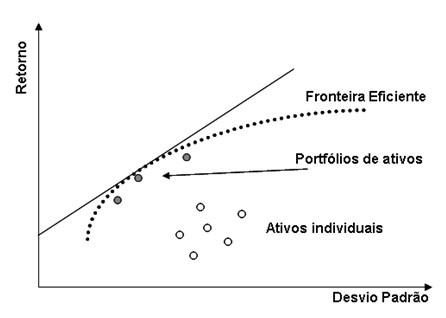
\includegraphics[height=4cm,keepaspectratio]{marko_02.png}
 \end{center}
 
\end{frame}


\begin{frame}{Minicaso}

\begin{itemize}
  \item IFN:  índice setor financeiro
  \item IMOB: índice do setor imobiliário
  \item ICON: índice de consumo
  \item IEE:  índice de energia
  \item INDX: índice da indústria
\end{itemize}

\end{frame}

\begin{frame}{Índices  IBOVESPA}

\begin{center}
 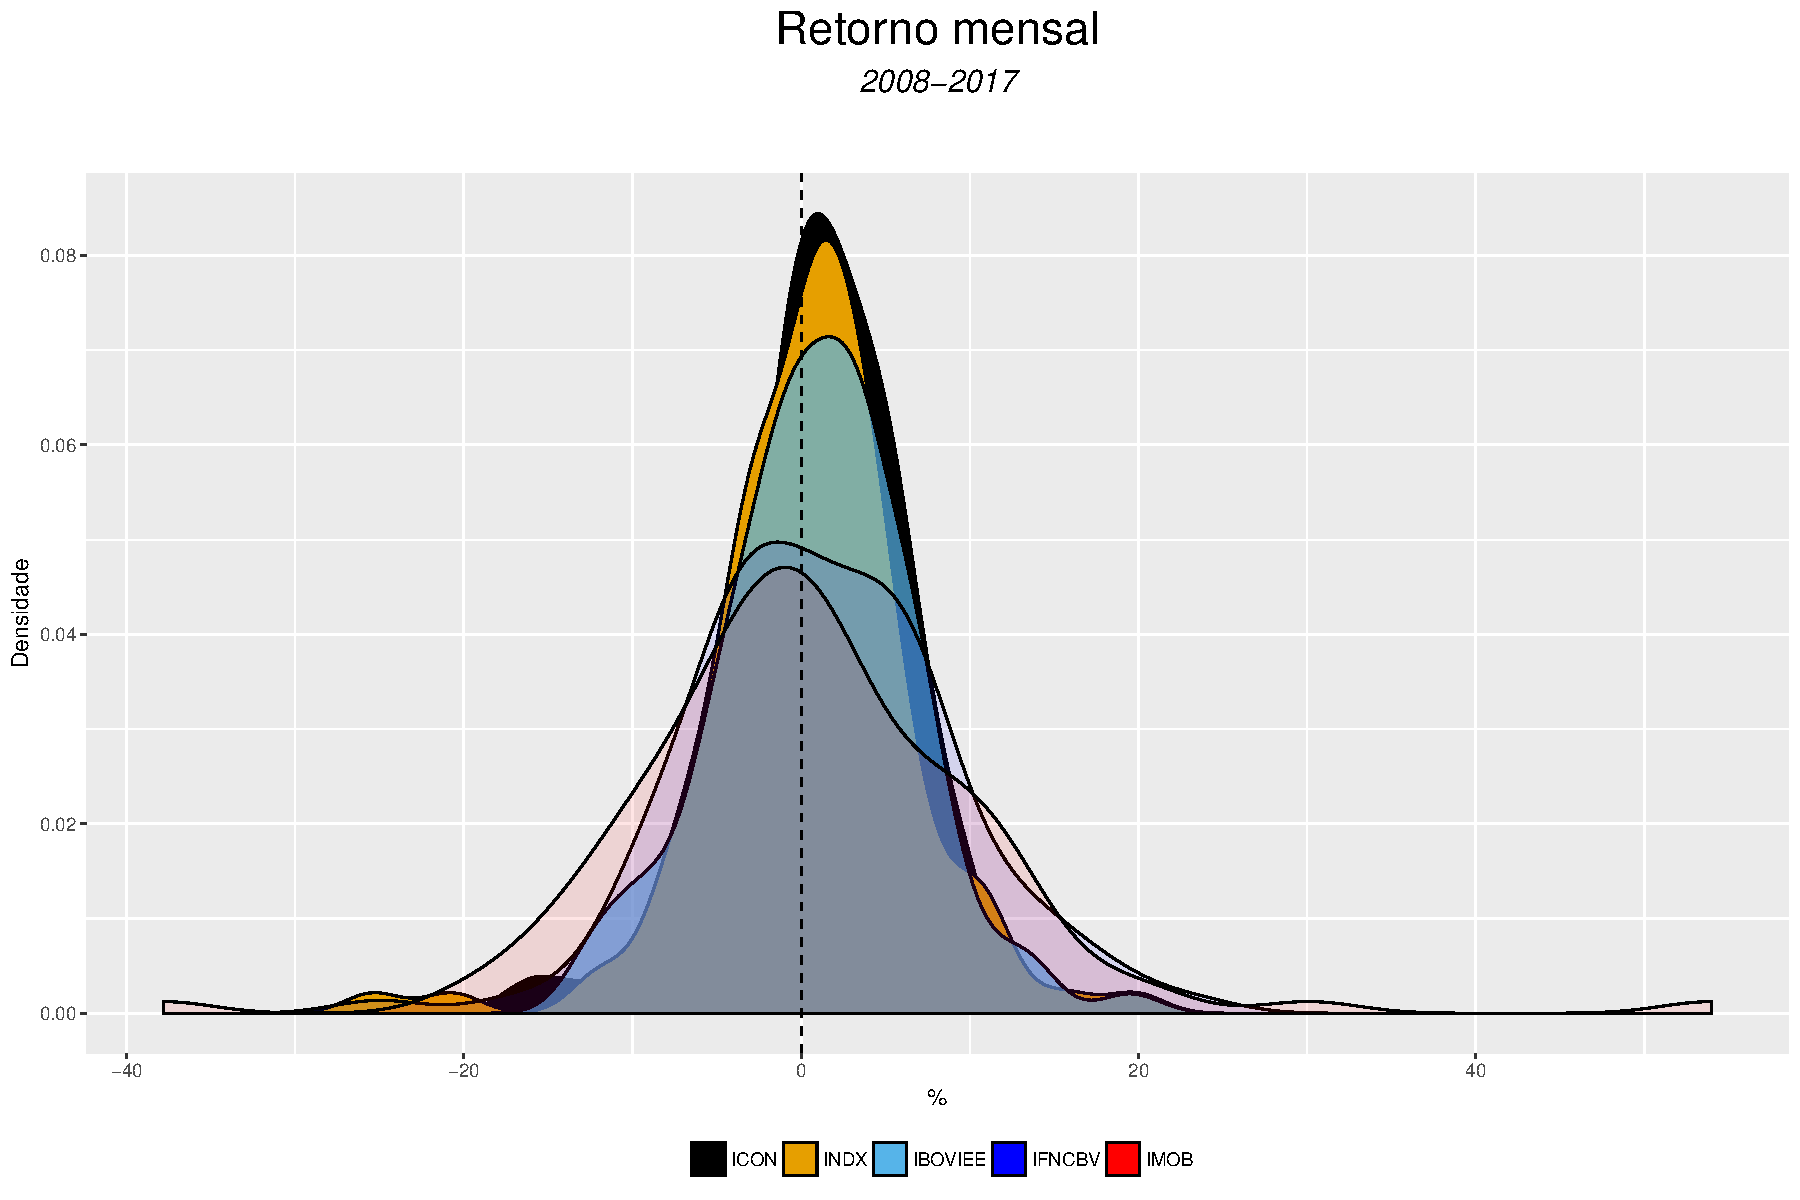
\includegraphics[height=8cm,keepaspectratio]{decritiva_indices.pdf}
 \end{center}


\end{frame}


\begin{frame}{Estatísticas}

\begin{center}
 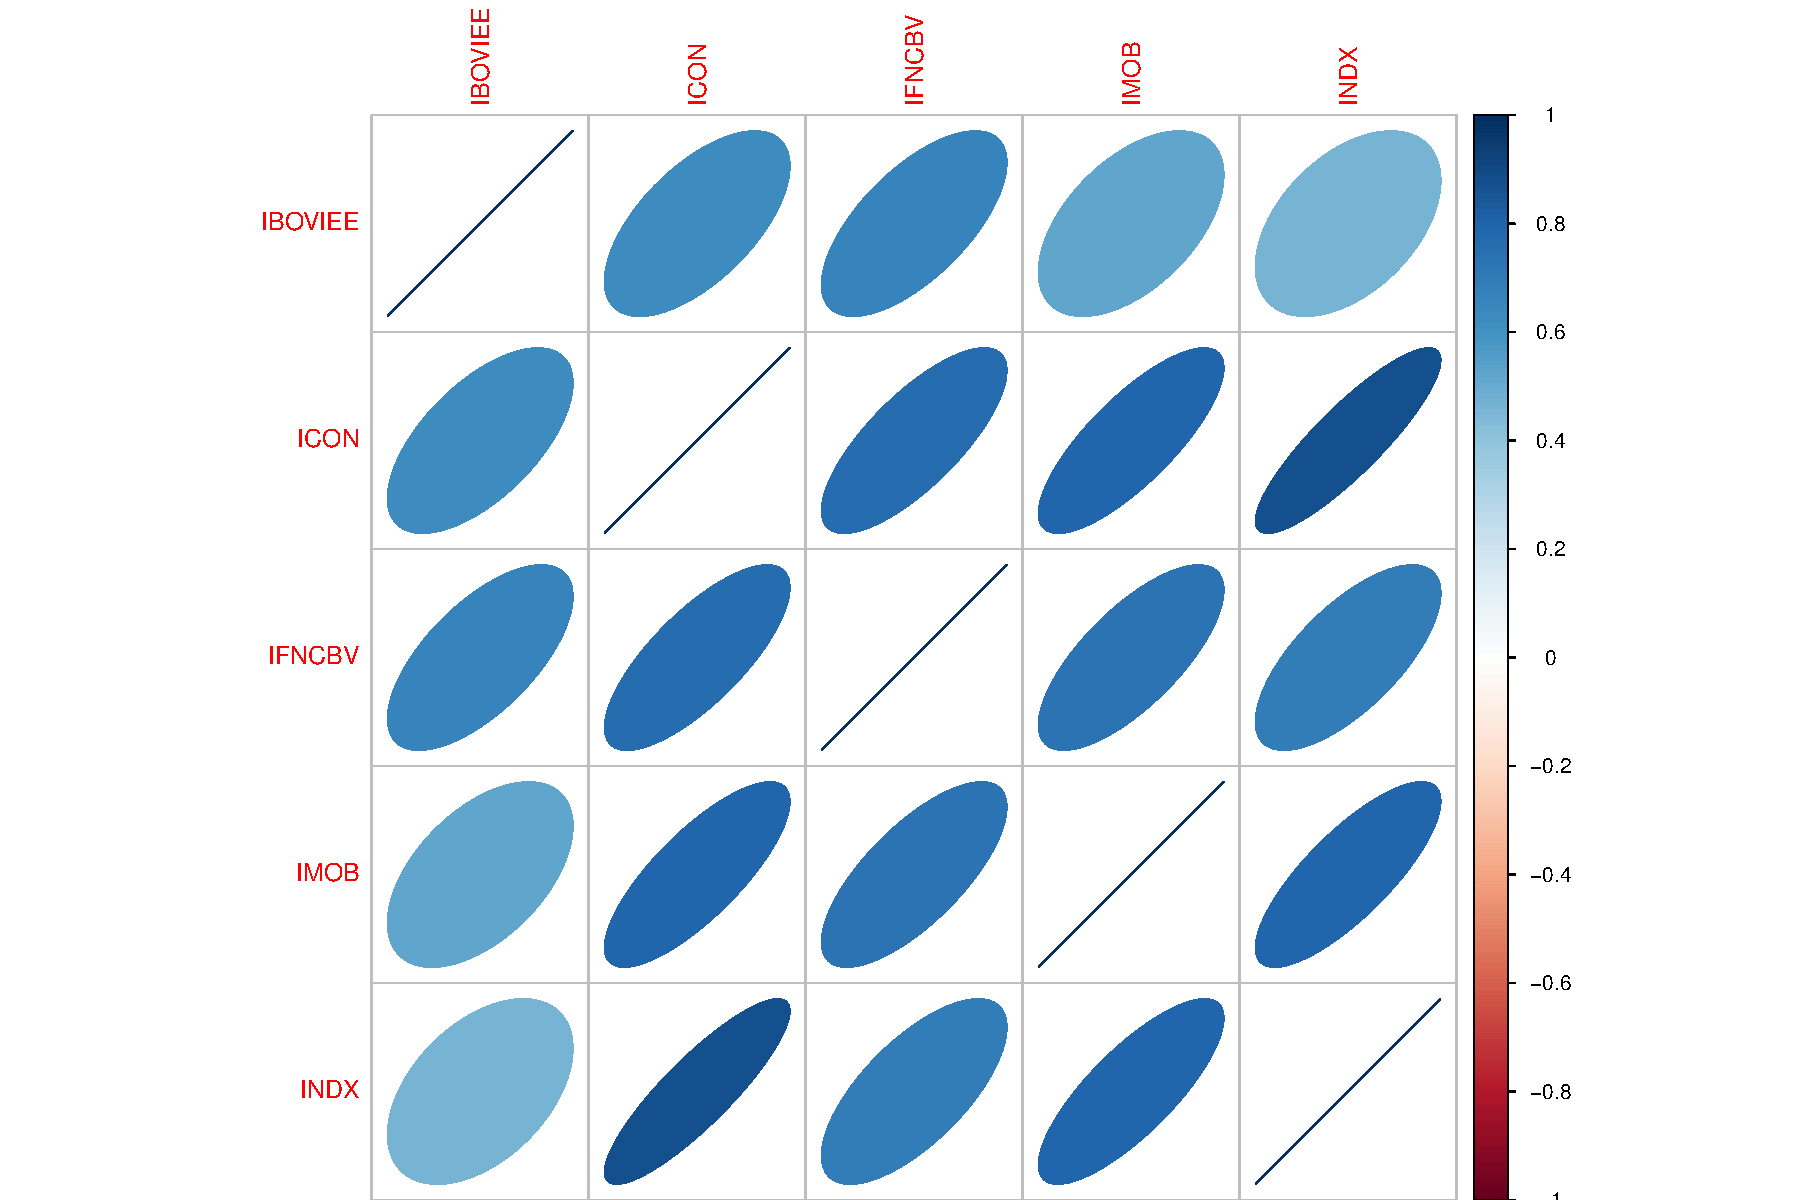
\includegraphics[height=8cm,keepaspectratio]{descritiva_cor.pdf}
 \end{center}


\end{frame}



\begin{frame}{Fronteira}

\begin{center}
 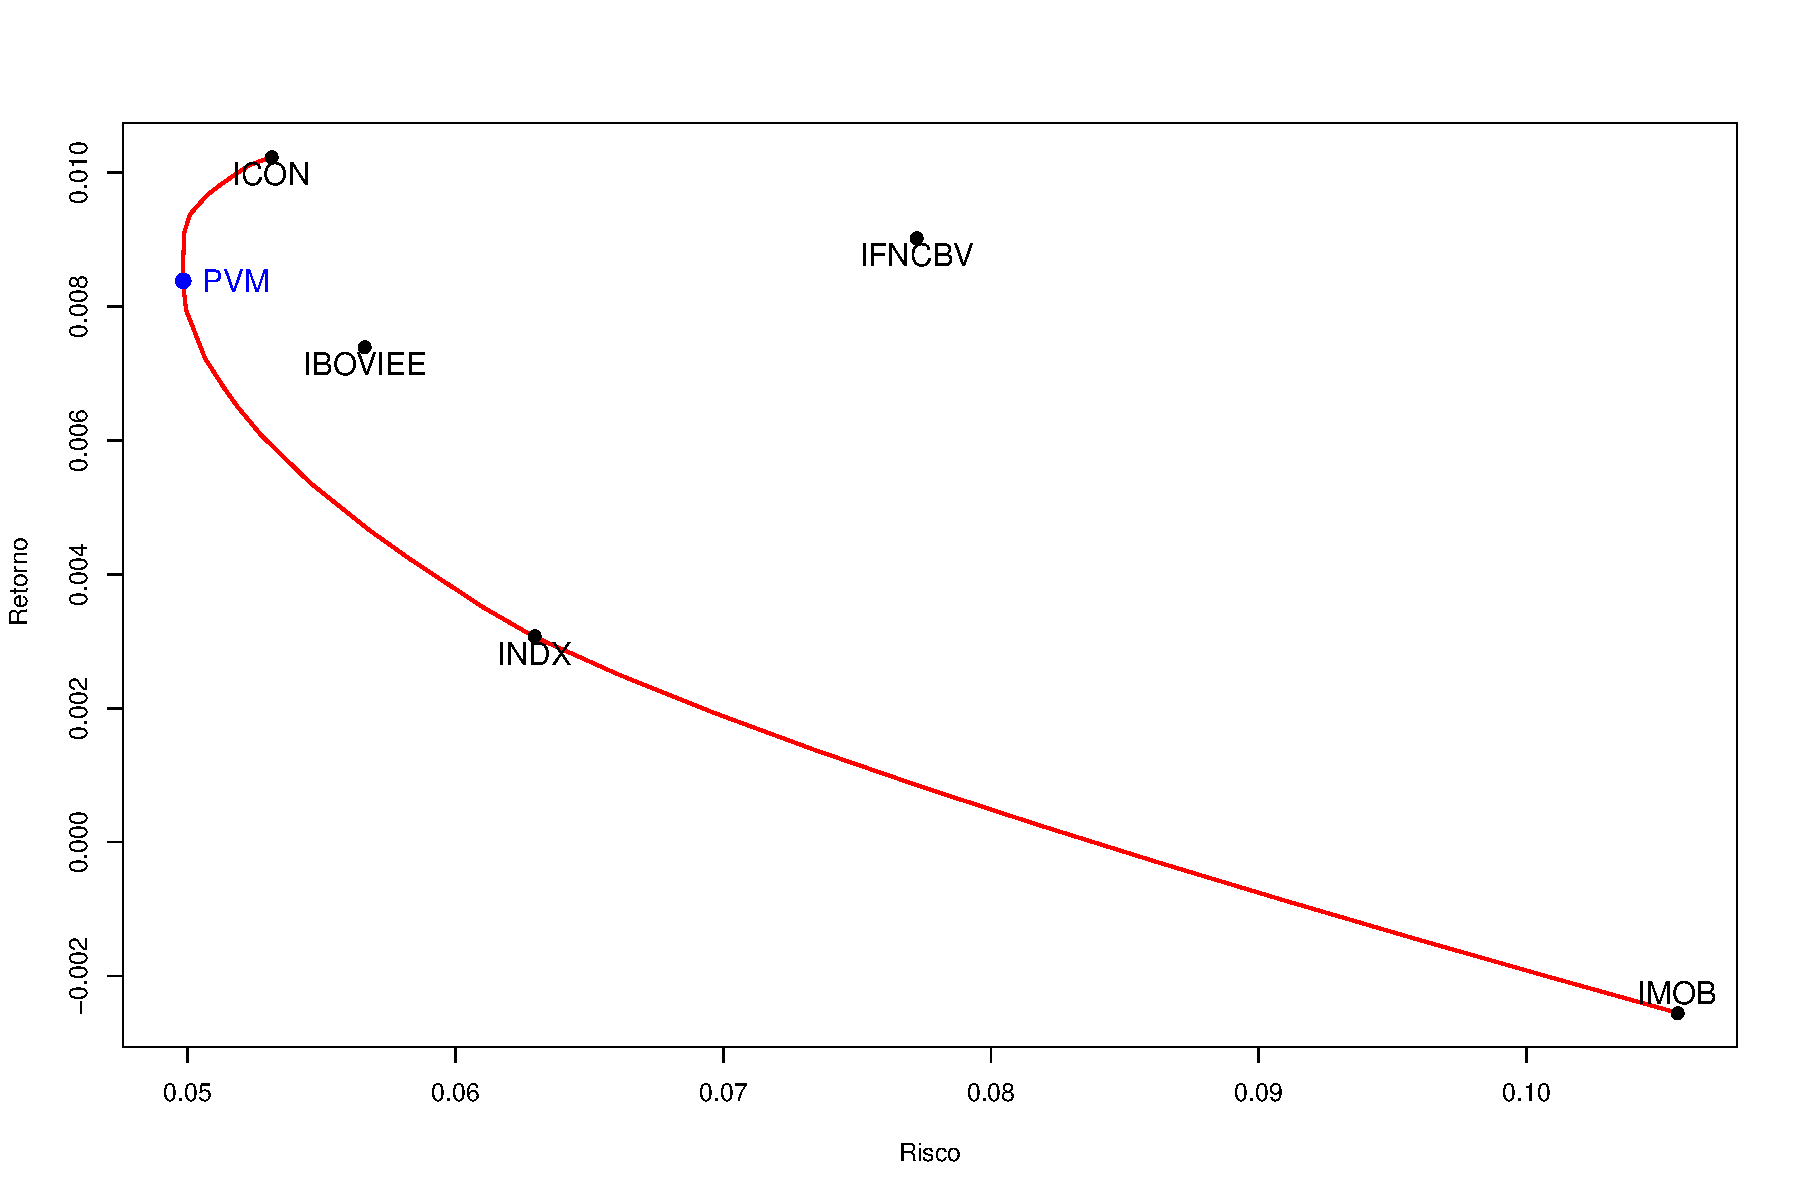
\includegraphics[height=8cm,keepaspectratio]{fronteira_ativos.pdf}
 \end{center}


\end{frame}


%\begin{frame}{Objetivo}
%
%Apresentar:
%
%\begin{itemize}
%\item Métodos numéricos para séries temporais 
%\item Desenvolvimentos recentes
%\item Principais aplicações
%\end{itemize}
%
%\end{frame}
%
%\begin{frame}{Expectativa ao final}
%
%\begin{itemize}
%\item Identificar diferenças entre os principais métodos
%\item Relacionar a aplicações em Finanças
%\item Conhecer referências clássicas e recentes na área
%\end{itemize}
%
%\end{frame}


\section{Stochastic Dynamic Programming}

\begin{frame}{ }
    \begin{block}{ }
      \Huge  Amostragem aleatória
    \end{block}
\end{frame}


\begin{frame}{Stochastic Dynamic Programming}

Um problema de programação dinâmica estocástica pode ser considerado, \citep{Consigli1998}:

\begin{enumerate}
\item um problema em múltiplos estágios recursivo;
\item um processo de decisões $d_t$ em $t=1,\cdots,T$;
\item com restrições conhecidas e parâmetros $w_t$ aleatórios. 
\end{enumerate}

\end{frame}



\begin{frame}{Stochastic Dynamic Programming}

Ao longo de todo o período $t=1,\cdots,T$, \citep{Kouwenberg2008}:

\begin{enumerate}
\item as decisões em $d_t$ estão intercaladas pelo que foi observado no instante $w_{t-1}$ e o que não se conhece sobre $w_{t}$
\item A relação entre a decisão tomada $d_{t-1}$ e o parâmetro de incerteza $w_{t-1}$ é \textbf{antecipativa} (condições de incerteza)
\item enquanto a relação entre $d_t$ e $w_{t-1}$ é \textbf{adaptativa} (ambiente de aprendizagem)
\end{enumerate} 

\end{frame}


\begin{frame}{Estrutura de decisão}
\begin{figure}
\begin{center}
 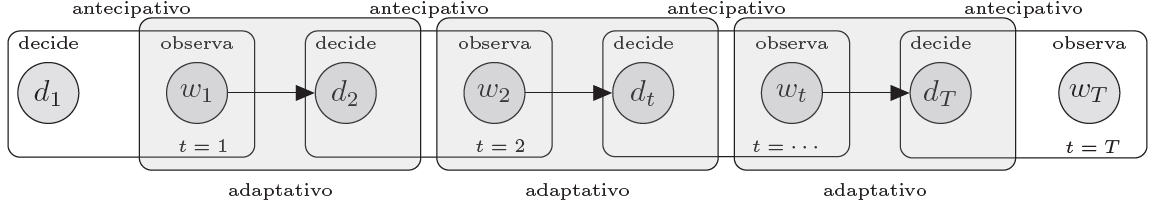
\includegraphics[height=2cm,keepaspectratio]{processo_adapt_antecipa.png}
 \end{center}
\label{fig:sadsad}
\end{figure}

\end{frame}




\begin{frame}{Estrutura de decisão}
\begin{equation}
\begin{array}{cc}
\left. \begin{aligned}
\text{Minimize:} \ \ &Z = f(d_t)  + E\left(q(d_t^{*},w_t)\right) \ \\
\text{Sujeito} \ \ & A d_t = \text{b} \\
& W(w_t)d_t^{*} = h(w_t) - T(w_t)d_t
 \end{aligned}\right.
\end{array}
\label{eq:fob}
\end{equation}


Otimizar, no instante $t$:
\begin{itemize}
\item  função $f(d_t)$ de custo formada pelo estágio antecipativo
\item e o valor esperado da função custo adaptativa $q(d_t^{*},w_t)$.
\end{itemize}
 
\pause 

\begin{enumerate}
\item  $A$: matriz tecnológica para $d_t$ 
\item $b$: vetor de recursos  para $d_t$ 
\item $T(w_t)$: matriz tecnológica que transforma $d_t$ em recursos $d_t^{*}$
\item $h(w_t)$: de recursos para $d_t^{*}$
\item $A$:matriz tecnológica para $d_t^{*}$
\end{enumerate}








\end{frame}



\begin{frame}{Cenário discretizado}

Discretizar o parâmetro de incerteza $w_t$ em \textbf{cenários}  $\Omega = \{w_t^{1},w_t^{2},\cdots,w_t^{N}\}$ \citep{Kouwenberg2008}.
\begin{itemize}
\item $p^{(l)} = \pi(w_t = w_t^{(l)})$
\item $\sum_{l=1}^N p^{(l)} = 1$
\end{itemize}

\begin{equation}
\begin{array}{cc}
\left. \begin{aligned}
\text{Minimize:} \ \ &Z = f(d_t)  +\sum_{l=1}^N p^{(l)} q(d_t^{*(l)},w_t^{(l)}) \ \\
\text{Sujeito} \ \ & A d_t = \text{b} \\
& W(w_t^{(l)})d_t^{*(l)} = h(w_t^{(l)}) - T(w_t^{(l)})d_t
 \end{aligned}\right.
\end{array}
\label{eq:fobc}
\end{equation}


\end{frame}



\begin{frame}{Estrutura de decisão}

\begin{enumerate}
\item O processo de otimização se repete dinamicamente a medida em que se tenha acesso a novas informações sobre $w_t$. 
\item A decisão $d_t^{*}$ no instante $t$ é a decisão $d_{t+1}$ do instante $t+1$.
\end{enumerate}

\begin{figure}
\begin{center}
 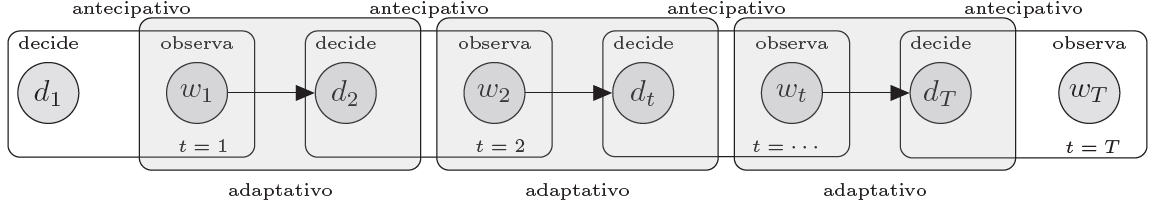
\includegraphics[height=2cm,keepaspectratio]{processo_adapt_antecipa.png}
 \end{center}
\label{fig:atcpt}
\end{figure}

\end{frame}







\begin{frame}{Função objetivo}


A função objetivo pode ser adaptada para:

\begin{itemize}
\item minimizar custo de administração \citep{Kouwenberg2008}
\item maximizar o valor final da carteira \citep{Johannes2014}
\item minimizar o risco \citep{Ferstl2011} e \citep{Quaranta2008}.
\end{itemize}

\end{frame}



\section{Amostragem aleatória (Intuitivo)}

\begin{frame}{ }
    \begin{block}{ }
      \Huge  Amostragem aleatória (Intuitivo)
    \end{block}
\end{frame}



\begin{frame}{Value at Risk (VaR)}

Definida a carteira ótima:

\begin{itemize}
\item em um dia ruim, quanto eu posso perder? 
\pause
\item quantos dias ruins eu suportaria para manter esse portfólio?
\end{itemize}

\end{frame}


\subsection{Monte Carlo }

\begin{frame}{ }
    \begin{block}{ }
      \Huge  Monte Carlo
    \end{block}
\end{frame}

\begin{frame}{Monte Carlo}

\begin{center}
 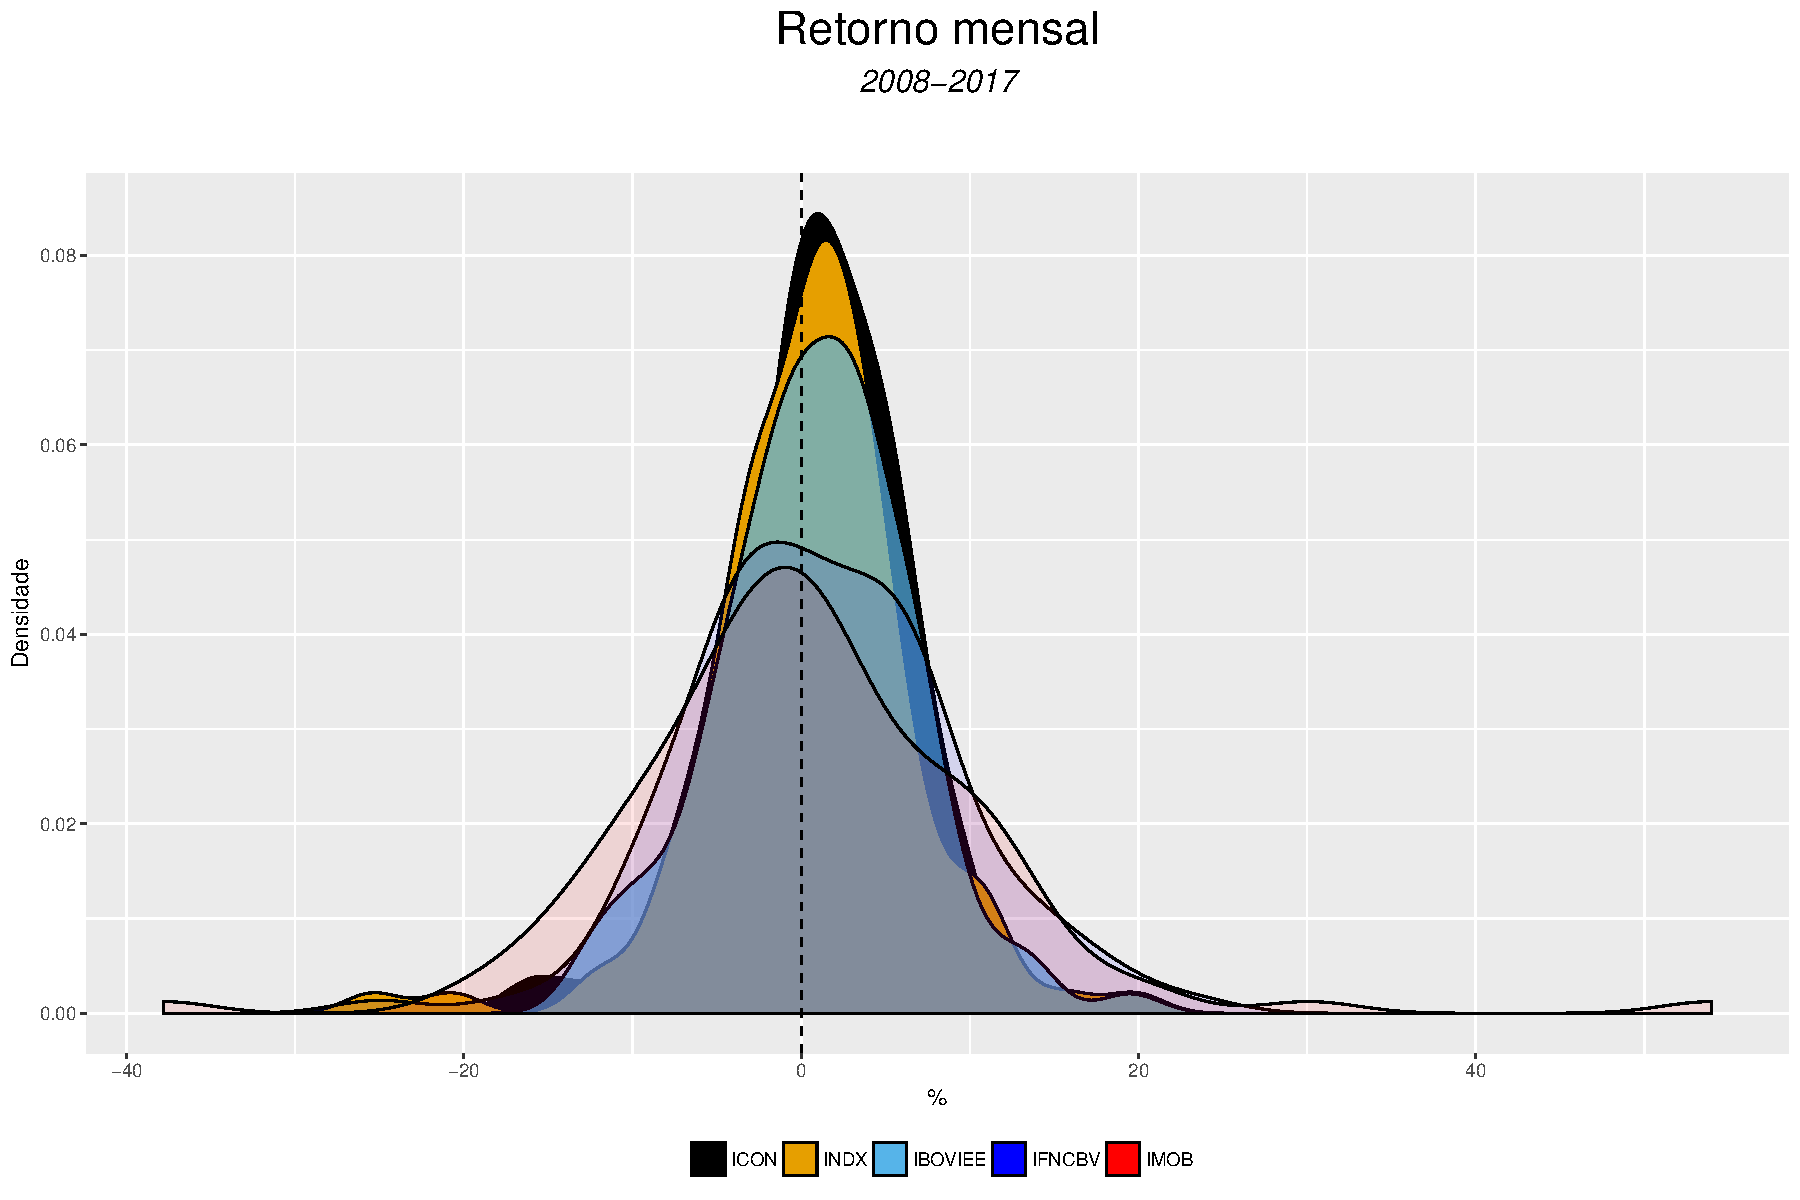
\includegraphics[height=8cm,keepaspectratio]{decritiva_indices.pdf}
 \end{center}

\end{frame}



\begin{frame}{Monte Carlo}

\begin{itemize}
\item descrição: (re)amostragem ``paramétrica"
\item vantagens: acessa ``todo" espaço
\item desvantagem: conhecimento prévio da distribuição
\end{itemize}

\end{frame}


\begin{frame}{Normal Multivariada}

\begin{equation*}
X \color{red}\sim N_k\left(\color{blue}\tilde{\mu}\color{red},\color{blue}\Sigma\color{red}\right)
\end{equation*}



\begin{equation*}
f(X) = \frac{1}{\sqrt{2\pi}}\frac{1}{\sqrt{det \color{blue}\Sigma}}exp\left(-\frac{1}{2}(\tilde{X}-\color{blue}\tilde{\mu}\color{black})\color{blue}\Sigma^{-1}\color{black}(\tilde{X}-\color{blue}\tilde{\mu}\color{black})\right)
\end{equation*}


\begin{enumerate}
\item \textcolor{red}{modelo}
\item \textcolor{blue}{parâmetros}
\item amostragem
\end{enumerate}


\end{frame}


\begin{frame}[fragile]{Code - MC}


\begin{verbatim}
set.seed(1052210218)
library(MASS)
n_mc <- 100000
mc <- mvrnorm(n=n_mc,mu,Sigma)
mc <- matriz_mc %*% w_optm
qlim <- quantile(mc,p=0.05)
   \end{verbatim}
\end{frame}

\begin{frame}{Value at Risk (Var)}

\begin{center}
 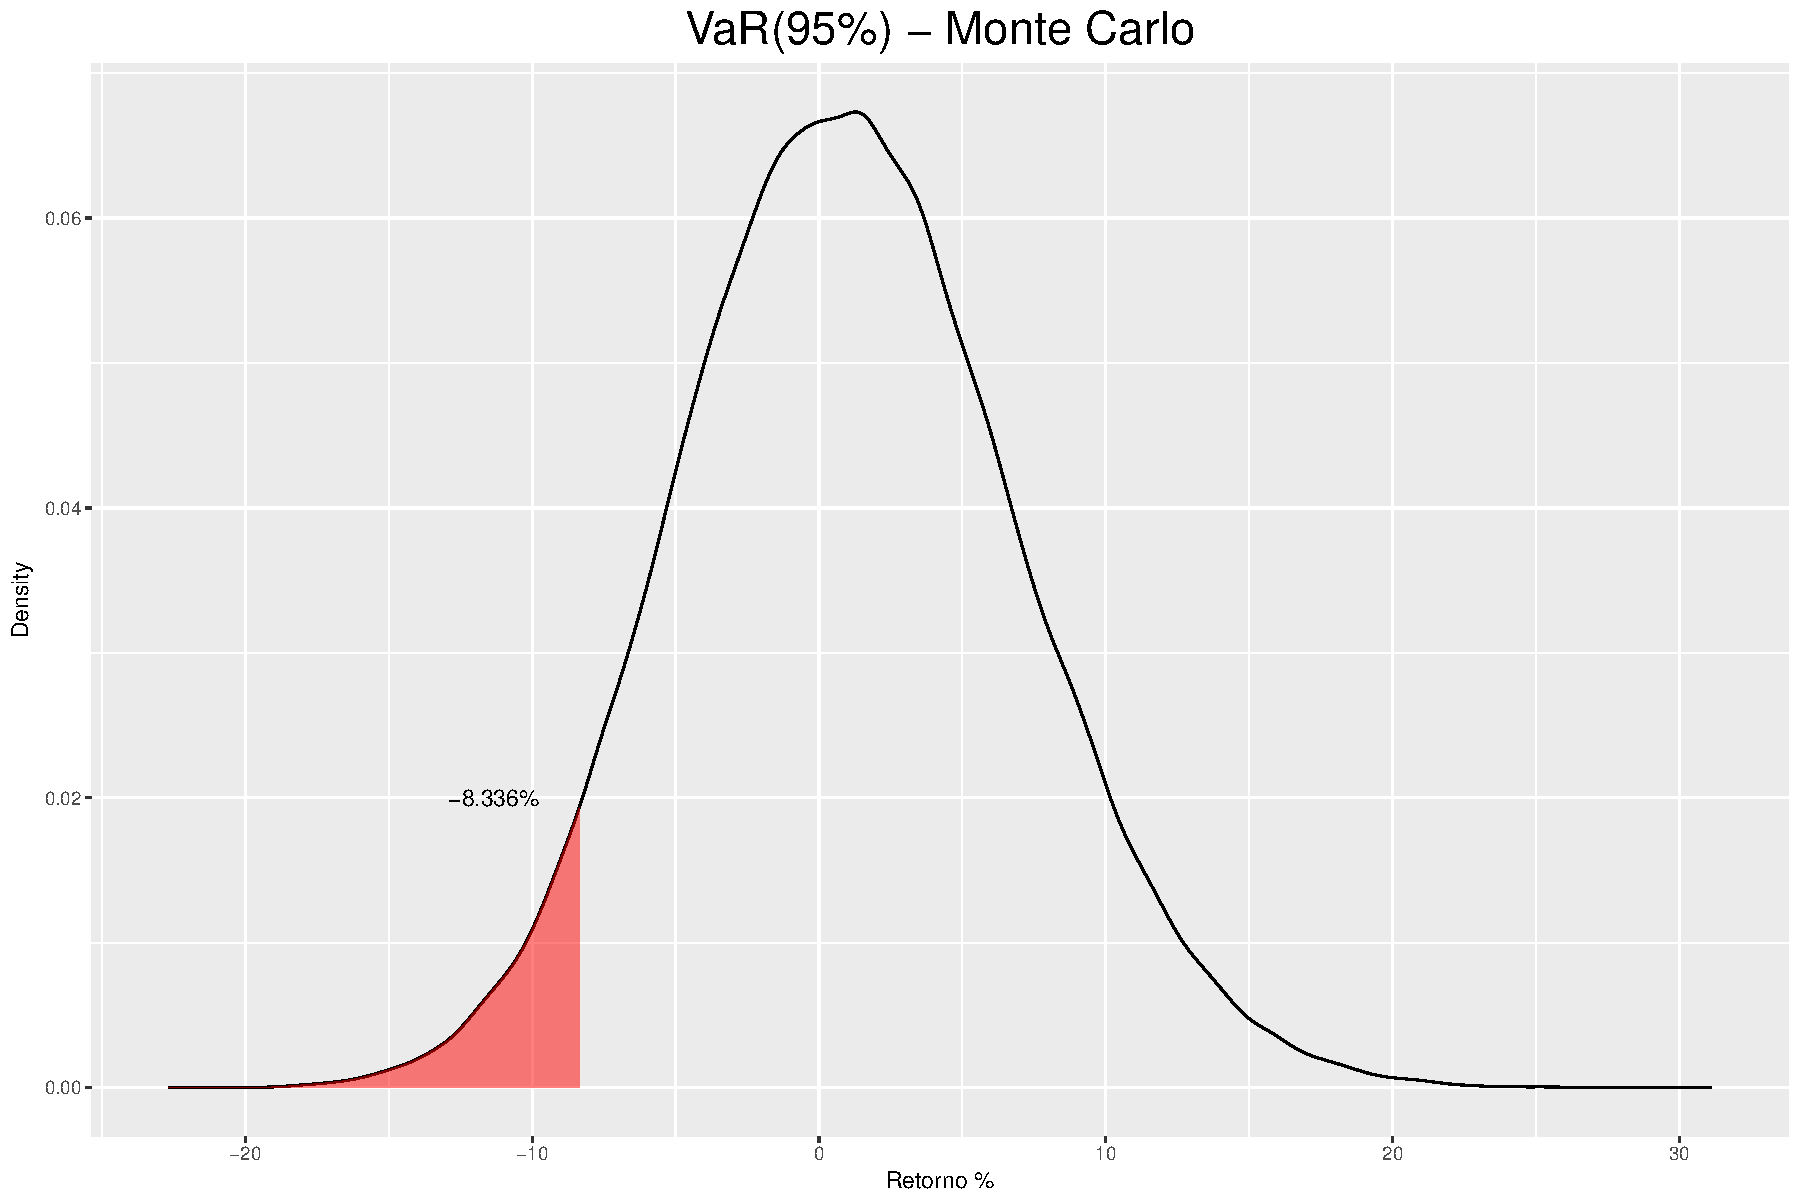
\includegraphics[height=8cm,keepaspectratio]{VAR_mc.pdf}
 \end{center}
 
\end{frame}

\begin{frame}{Pontos importantes}
\begin{itemize}
\item Suposição da distribuição:
\item Estrutura de dependência longitudinal?
\end{itemize}
\end{frame}

\subsection{Bootstrap}

\begin{frame}{ }
    \begin{block}{ }
      \Huge  Bootstrap
    \end{block}
\end{frame}



\begin{frame}{ Bootstrap}


\begin{itemize}
\item descrição: (re)amostragem ``não-paramétrica"
\item vantagens: não requer conhecimento sobre a distribuição
\item desvantagem: acessa espaço ``realizado"
\end{itemize}

\pause

\begin{itemize}
\item Suposição da distribuição: amostragem aleatória nos próprios dados
\item Estrutura de dependência longitudinal: Base divida em janelas $5$ meses
\end{itemize}
 
\end{frame}




\begin{frame}{Value at Risk (Var) - Bootstrap}

\begin{center}
 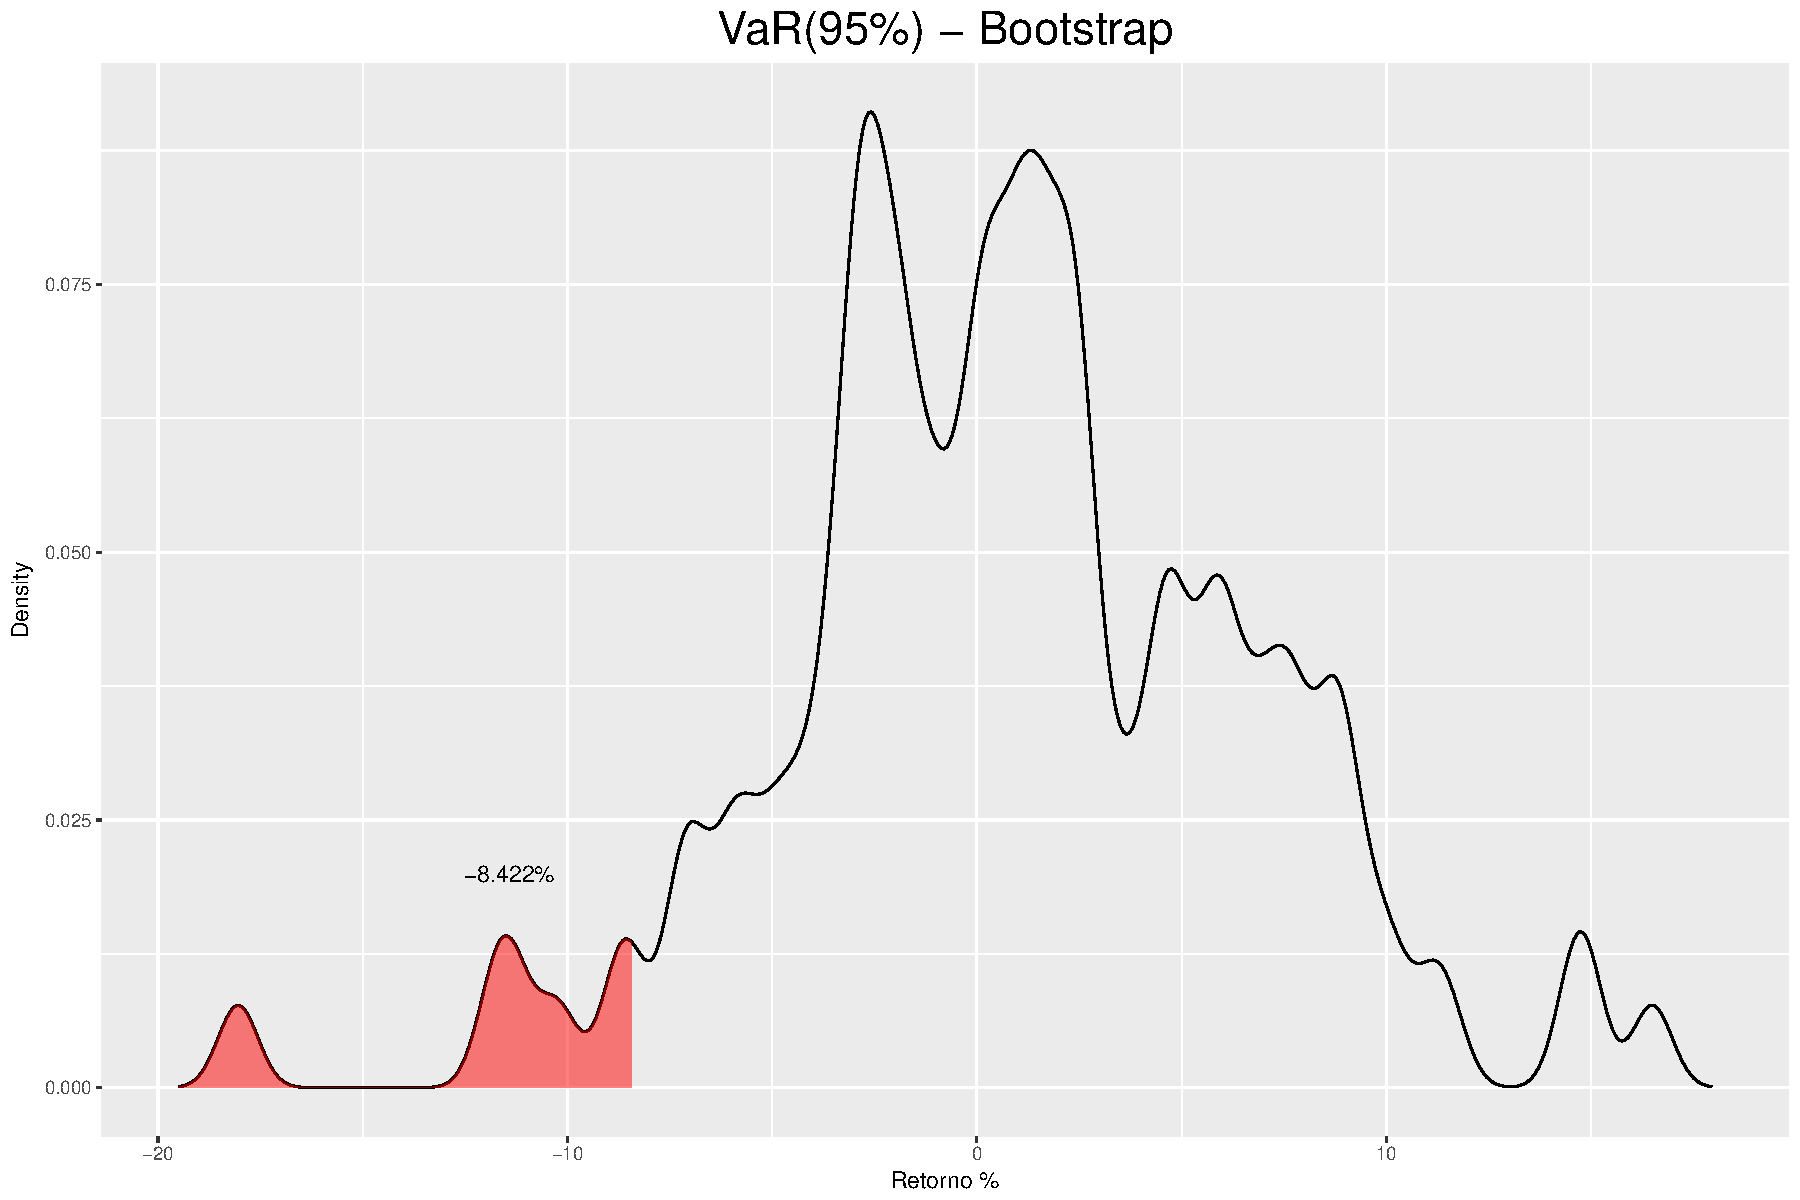
\includegraphics[height=8cm,keepaspectratio]{VAR_boots.pdf}
 \end{center}
 
\end{frame}



\section{Modelos Dinâmicos}


\begin{frame}{ }
    \begin{block}{ }
      \Huge  Modelos Dinâmicos
    \end{block}
\end{frame}


\begin{frame}{Modelo dinâmico}
\noindent

 
  \begin{block}{Parte não observável - sistema}
  {\large Sequência $\theta_t$ com estrutura de dependência de um Processo Markoviano, $\{\theta_t$, $t=1,...,n\}$.}
\end{block}

\pause
  \begin{block}{Parte observável}
  {\large Sequência $y_t$ $\{y_t$, $t=1,...,n\}$ que é dependente, exclusivamente, de $\theta_t$.}
\end{block}
  

\end{frame}


\begin{frame}{Modelo dinâmico}
\only<1>{	
  \begin{center}
  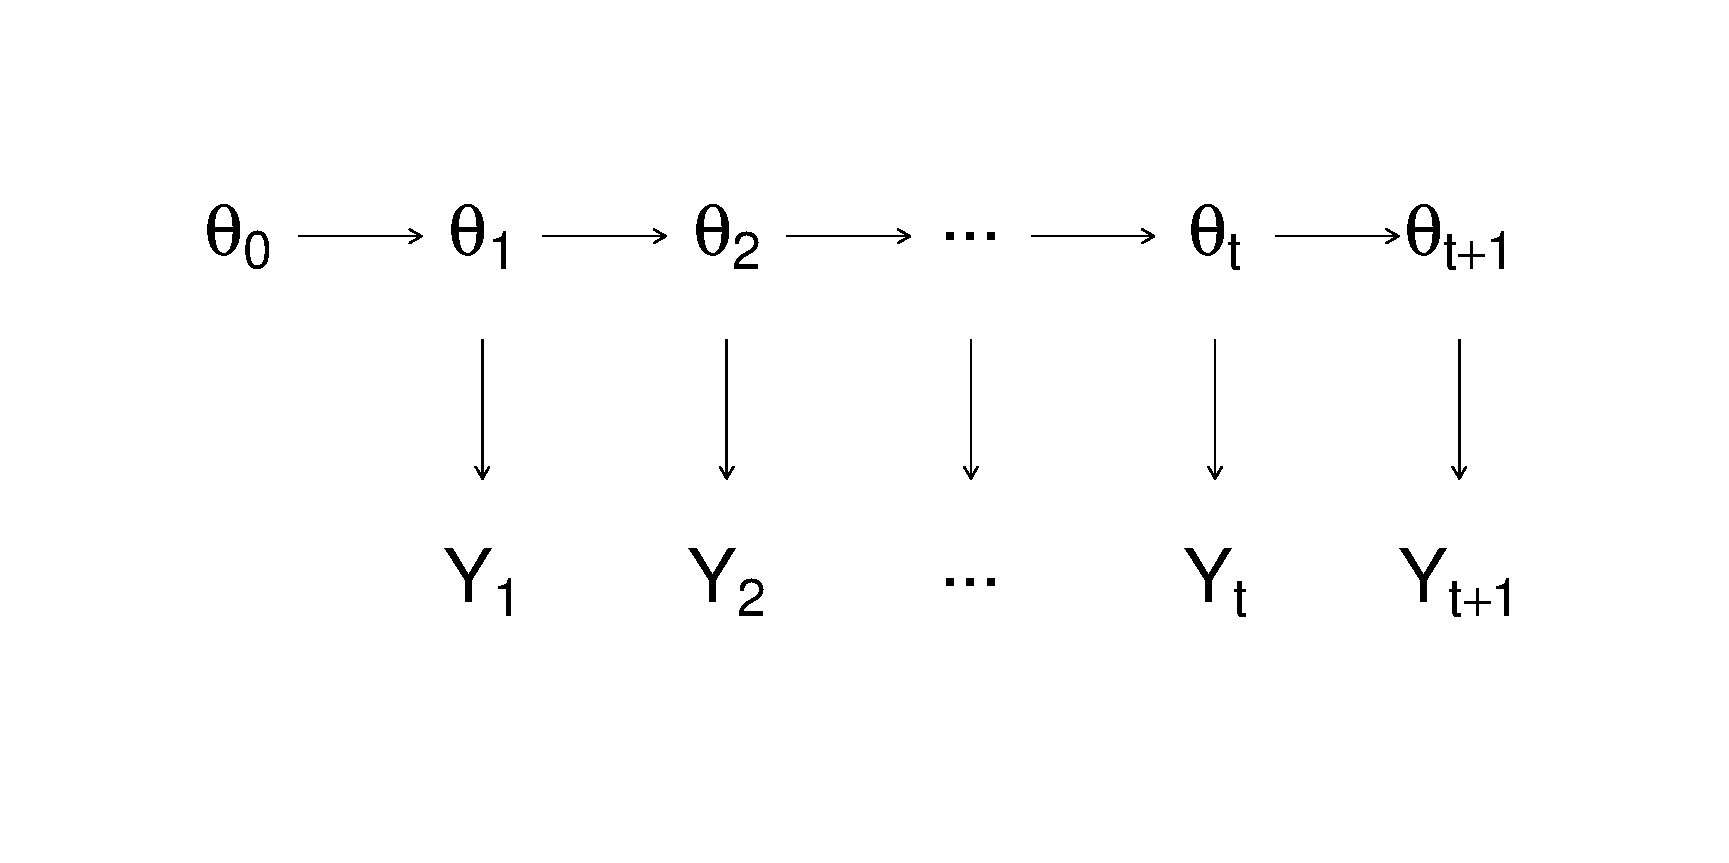
\includegraphics[height=4cm,keepaspectratio]{modelodinamicoR.pdf}
  \end{center}
}
\only<2>{
  \begin{center}
  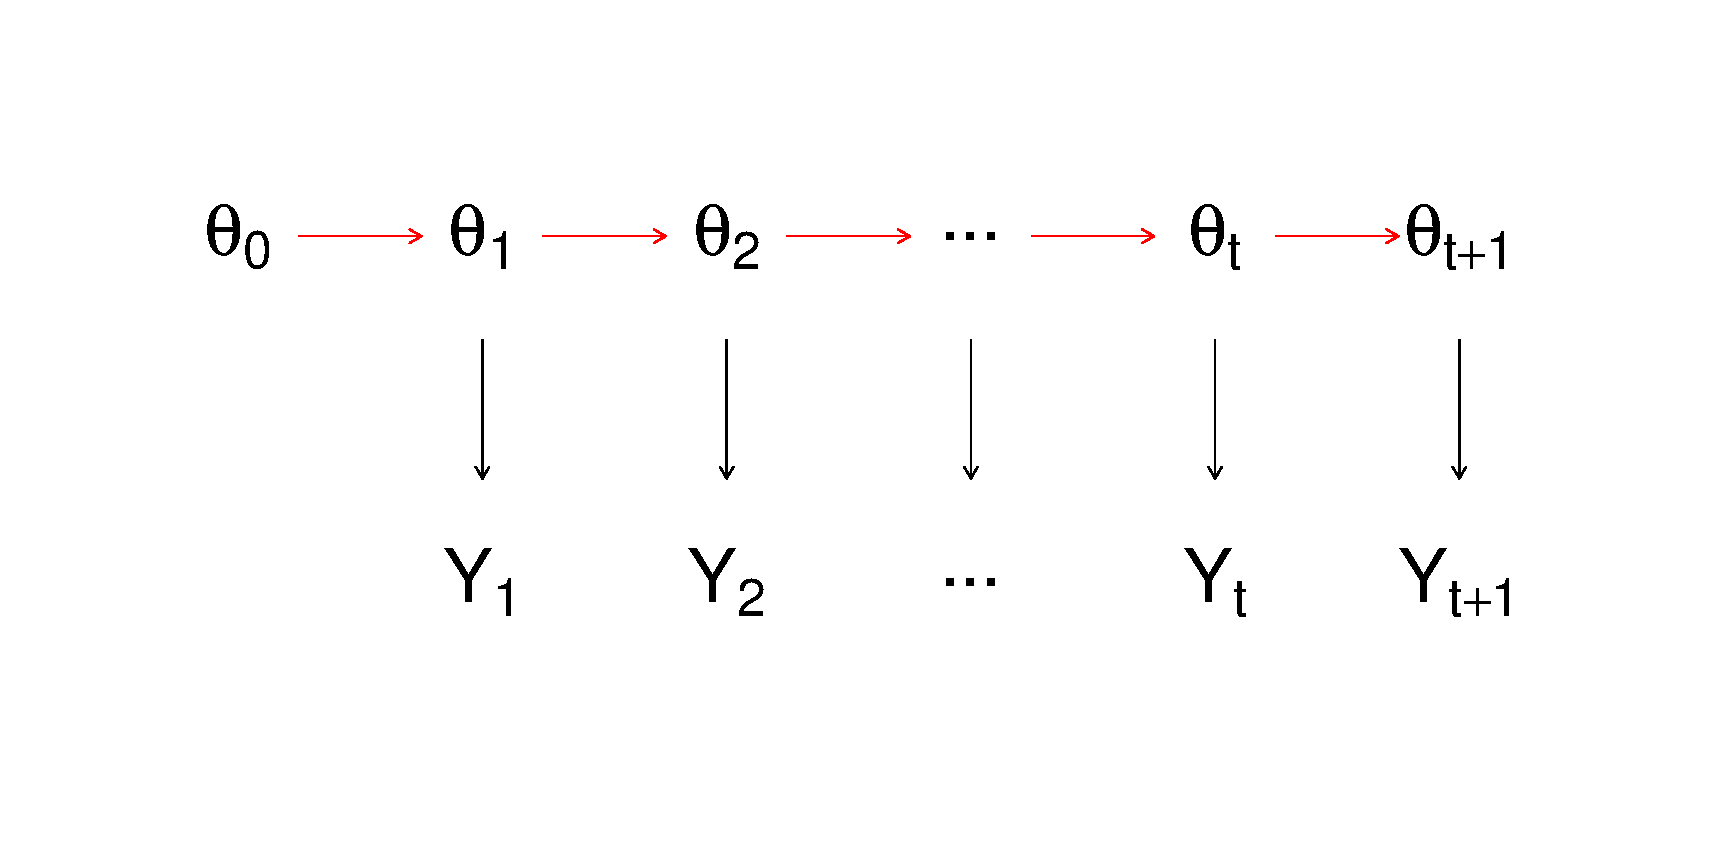
\includegraphics[height=4cm,keepaspectratio]{modelodinamicoR1.pdf}
  \end{center}
}
\only<3>{
  \begin{center}
  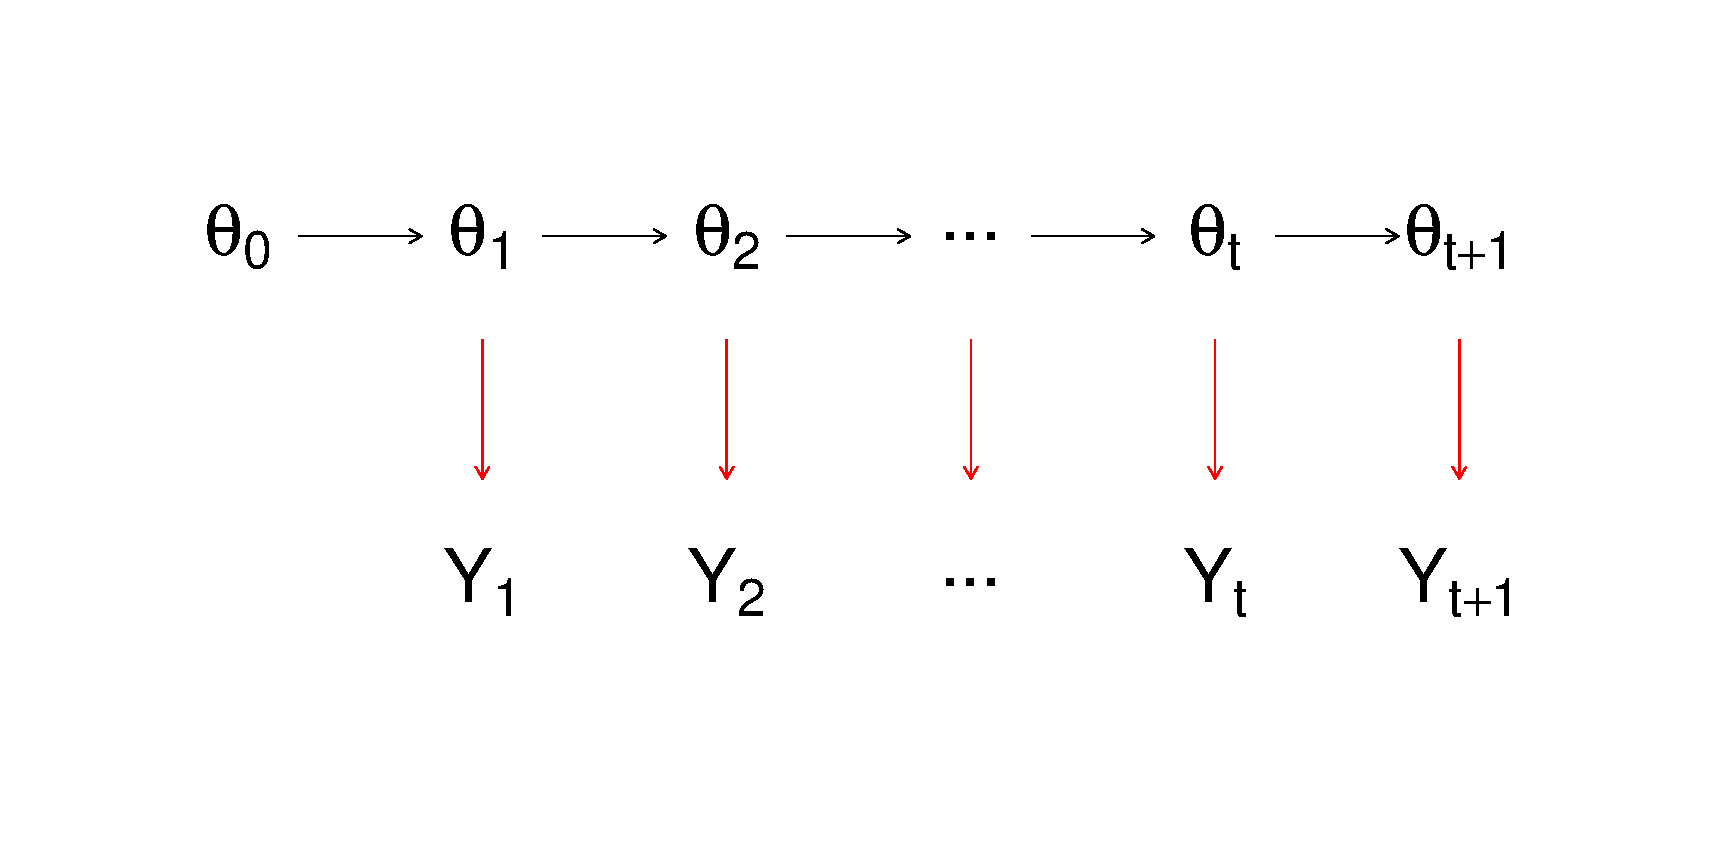
\includegraphics[height=4cm,keepaspectratio]{modelodinamicoR2.pdf}
  \end{center}
}
\pause
\underline{\textbf{Equação do Sistema}}
$$
\theta_t =  G_t \theta_{t-1} + w_t
$$
\pause
\underline{\textbf{Equação das Observações}}
$$
y_t  =  F_t \theta_{t} + v_t
$$

\end{frame}

\begin{frame}{Propriedades}
\begin{center}
\begin{itemize}
\item[A.1:] $\theta_t, t=1,...,n$ é uma sequência de estados de um Processo Markoviano;

$$
\pi(\theta_{1:n}) = \pi(\theta_1) \prod_{k=2}^n \pi(\theta_k|\theta_{k-1}) 
$$

\pause 

\item[A.2:] $y_{1:t}$ é um vetor de observações que são condicionalmente independentes dado $\theta_{1:t}$, para cada $t=1,...,n$.

$$
\pi(y_t|\theta_{1:t},y_{1:t-1}) = \pi(y_t|\theta_{t})
$$

\end{itemize}
\end{center}
\end{frame}


\begin{frame}{Distribuição conjunta}

Essas propriedades permitem descrever a \textbf{distribuição conjunta} das observações e dos estados como o produto das seguintes \textbf{distribuições condicionais}:

$$
\pi(y_{1:n},\theta_{1:n}) = \pi(\theta_0) \prod_{t=1}^n \pi(\theta_t|\theta_{t-1})\pi(y_t|\theta_t) 
$$

\underline{\textbf{Interesse:}}

$$\pi(\theta_{1:n}|y_{1:n}) =  \frac{\pi(\theta_{1:n},y_{1:n})}{\pi(y_{1:n})} $$


\end{frame}


\begin{frame}{Filtro de Kalman}

Seja $v_t$ e $w_t$ perturbações com distribuição Gaussiana e independentes, \cite{west} apresenta um esquema sequencial para o processo de filtragem, conhecido como \textbf{Filtro de Kalman}.

\begin{itemize}
\item[(a)]\textbf{\textit{Posteriori} de $\theta$ em $t-1$}:  $(\theta_{t-1}|D_{t-1})\sim N[m_{t-1},C_{t-1}]$;
\item[(b)]\textbf{Atualização da \textit{priori} em $t-1$:} $(\theta_{t}|D_{t-1})\sim N[m_{t-1},R_{t}]$;
\item[(c)]\textbf{Predição para $y$ em $t$:}  $(y_t|D_{t-1})\sim N[f_{t},Q_{t}]$;
\item[(d)]\textbf{Posteriori de $\theta$ em $t$:}  $(\theta_t|D_{t})\sim N[m_{t},C_{t}]$;
\end{itemize}
Sendo: $R_t = C_{t-1}+W_t$, $f_t = m_{t-1}$, $Q_t = R_{t}+V_t$, $\theta_t = m_{t-1}+A_te_t$,  $C_t=A_tV_t$, $A_t=R_t/Q_t$ e $e_t=Y_t-f_t$.

\end{frame}


\subsection{Monte Carlo}

\begin{frame}{Amostragem aleatória}

    \begin{block}{}
      \Huge  Monte Carlo (formal)
    \end{block}


\end{frame}

\begin{frame}{Definição}

\textbf{Distribuição alvo} : $\pi_n(\theta_1,...,\theta_n)$ para $n$ fixo.

\pause
\vspace{0.5cm}

Gera-se $N$ amostras independentes da variável aleatória $\Theta^i_{1:n} \sim \pi_n(\theta_1,...,\theta_n)$, $i=1,...,N$.

\pause
\vspace{0.5cm}

Aproximação e dada por:

$$
\hat{\pi}_n(\theta_1,...,\theta_n) = \frac{1}{N}\sum_i^N \delta_{\Theta^i_{1:n}}(\theta_{1:n}),
$$

\vspace{0.5cm}
sendo $\delta_{\Theta_{1:n}^{i}}(\theta_{1:n})$ uma função indicadora de massa no ponto $\theta_{1:n}$.
\end{frame}



\begin{frame}{Definição}

Considerer mensurar uma função $\phi_n$ em $\pi(\theta_1,...,\theta_n)$:

$$
E(\phi_n) =  \int \phi_n(\theta_1,...,\theta_n)\pi_n(\theta_1,...,\theta_n)d\theta_{1:n}
$$
\pause

Pelo método Monte Carlo, \textbf{avaliamos}  $\phi_n$ no suporte simulado de $\pi(\theta_1,...,\theta_n)$ por meio das \textbf{amostras}:

$$
\hat{E}(\phi_n) = \int \phi_n(\theta_1,...,\theta_n)\hat{\pi}_n(\theta_1,...,\theta_n)d\theta_{1:n}
$$
\pause
$$
\hat{E}(\phi_n) = \frac{1}{N} \sum_{i=1}^N \phi_n(\Theta^i_{1:n})
$$


\end{frame}

\begin{frame}{Desvantagens}


\begin{itemize}

\item[] \underline{\textbf{Problema 1}}: Não é fácil se gerar $\pi_n(\theta_1,...,\theta_n)$. 
\pause 

\vspace{.5cm}
\item[] \underline{\textbf{Problema 2}}: Ainda que fosse possível se gerar, a dimensão de $\pi_n(\theta_1,...,\theta_n)$ pode ser muito grande para se obter amostras multivariadas. Problema encontrado no método \underline{\textbf{MCMC}}. 

\end{itemize}
\end{frame}


\subsection{Amostragem de Importância - AI}

\begin{frame}{Problema 1}
    \begin{block}{}
      \Huge  Amostragem de importância
    \end{block}
\end{frame}


\begin{frame}{Problema 1}

A amostragem de importância trata o \textbf{\underline{problema 1}}: não se sabe gerar $\pi(\theta_{1:n})$.

\vspace{0.5cm}
\pause

Utiliza-se uma \textbf{distribuição de importância} $q(.)$ para obter o mesmo suporte da distribuição $\pi(.)$ .
$$
E_{\pi}(\phi)=\int \phi(\theta) \pi(\theta) d\theta = \int \frac{ \phi(\theta) \pi(\theta)}{q(\theta)} q(\theta) d\theta
$$

\pause
A quantidade $\frac{\pi(\theta)}{q(\theta)}$  fornece um ajuste da discrepância entre \textbf{gerar um suporte} de $\pi(\theta)$ por meio da distribuição geradora $q(\theta)$.

\end{frame}



%%
%%\begin{frame}{Notação}
%%
%%Considere a seguinte representação, \cite{doucet2}:
%%$$ \pi(\theta_{1:n}) = \frac{\gamma_n(\theta_{1:n})}{Z_n(\theta_{1:n})}, \hspace{1cm} Z_n = \int \gamma_n(\theta_{1:n}) d\theta_{1:n}$$
%%
%%\pause
%%
%%Considere uma distribuição auxilar, tal que:
%%
%%$$ \pi(\theta_{1:n}) > 0 \rightarrow q_n(\theta_{1:n})>0$$
%%
%%
%%\end{frame}



%
%\begin{frame}{Peso}
%
%\underline{A distribuição de interesse}:
%\begin{tabular}{ccc}
%$ \pi(\theta_{1:n}) = \frac{\gamma_n(\theta_{1:n})}{Z_n(\theta_{1:n})}= $  & $ \overbrace{ \frac{\gamma_n(\theta_{1:n})}{q_n(\theta_{1:n})} }^{W_n} $  & $ \frac{q_n(\theta_{1:n})}{Z_n(\theta_{1:n})} $
%\end{tabular}
%
%\vspace{0.5cm}
%$$ \pi(\theta_{1:n}) = \frac{w_n(\theta_{1:n})q_n(\theta_{1:n})}{Z_n(\theta_{1:n})} $$
%
%\pause
%
%O denominador é:
%
%$$ Z(\theta_{1:n}) = \int w_n(\theta_{1:n})q_n(\theta_{1:n})d\theta_{1:n}$$
%
%\end{frame}
%
%
%
%\begin{frame}{Aproximação}
%
%Considere $N$  amostras independentes $\Theta^i_{1:n} \sim q_n(\theta_{1:n})$.
%
%\pause
%\vspace{0.5cm}
%
%Aproximação Monte Carlo é:
%
%$$
%\hat{q}_n(\theta_{1:n}) = \frac{1}{N} \sum^N_i \delta_{\Theta^i}(\theta_{1:n})
%$$
%
%\vspace{0.5cm}
%
%Dessa forma, a aproximação para a distribuição de interesse é:
%
%\pause
%
%$$
%\hat{\pi}_n(\theta_{1:n}) = \frac{w_n(\theta_{1:n})\hat{q}_n(\theta_{1:n})}{\int w_n(\theta_{1:n})\hat{q}_n(\theta_{1:n}) d\theta_{1:n}}
%$$
%
%
%\end{frame}
%
%
%
%
%\begin{frame}{Aproximação}
%
%A distribuiçao de interesse pode ser expressa por:
%
%$$\hat{\pi}_n(\theta_{1:n})= \frac{\frac{1}{N} \sum^N_{i=1} w_n(\Theta^i_{1:n})\delta_{\Theta^i_{1:n}}(\theta_{1:n})}{ \int  w_n(\theta_{1:n})\left[ \frac{1}{N} \sum^N_{i=1} \delta_{\Theta^i_{1:n}}(\theta_{1:n}) \right] d\theta_{1:n}} $$
%
%\pause
%
%
%$$\hat{\pi}_n(\theta_{1:n})= \frac{ \sum^N_{i=1} w_n(\Theta^i_{1:n})\delta_{\Theta^i_{1:n}}(\theta_{1:n})}{   \sum^N_{i=1} w_n(\Theta^i_{1:n})\left[ \int \delta_{\Theta^i_{1:n}}(\theta_{1:n}) d\theta_{1:n} \right] }, $$
%
%\pause
%sendo,
%$$ \int \delta_{\Theta^i_{1:n}}(\theta_{1:n}) d\theta_{1:n} =1 $$
%
%$$\hat{Z}_n(\theta_{1:n})=    \sum^N_{i=1} w_n(\Theta^i_{1:n}) $$
%
%
%\end{frame}
%


\begin{frame}{Aproximação}

Dessa forma,
$$\hat{\pi}_n(\theta_{1:n})= \frac{\sum^N_{i=1} w_n(\Theta^i_{1:n})\delta_{\Theta^i_{1:n}}(\theta_{1:n})}{\sum^N_{i=1} w_n(\Theta^i_{1:n})} $$

\pause

Sendo:

$$W_n(\theta_{1:n})= \frac{ w_n(\Theta^i_{1:n})}{ \sum^N_{j=1} w_n(\Theta^j_{1:n})} $$

\pause

$$\hat{\pi}_n(\theta_{1:n})= \sum^N_{i=1} W_n(\Theta^i_{1:n})\delta_{\Theta^i_{1:n}}(\theta_{1:n}) $$

\pause
A aproximação Monte Carlo para a função $\phi_n(.)$ é:
$$
\hat{E}(\phi_n) = \frac{1}{N} \sum_{i=1}^N W_n(\Theta^i_{1:n}) \phi_n(\Theta^i_{1:n}).
$$

\end{frame}


\subsection{Amostragem de Importância Sequencial - (AIS)}

\begin{frame}{Problema 2}
    \begin{block}{}
      \Huge  Amostragem de importância sequencial (AIS)
    \end{block}
\end{frame}




\begin{frame}{Problema 2}

Apesar do uso da amostragem de importância, amostrar $q_n(\theta_{1:n})$ pode ser \textbf{inviável devido a dimensão} $n$.

\vspace{0.5cm}

\pause

Considere que a distribuição auxiliar escolhida, $q(.)$, possa ser escrita por:
$$ q(\theta_{1:n})  = q(\theta_{1:n-1})q(\theta_n|\theta_{1:n-1})$$

\vspace{0.5cm}

\pause
Tem-se:

$$ q(\theta_{1:n})  = q(\theta_1)\prod_{k=2}^n q(\theta_k|\theta_{1:k-1})$$

\end{frame}




%
%\begin{frame}{Decomposição sequecial}
%Assim, os pesos no tempo $t=2$:
%$$
%w(\theta_{1:2}) =\frac{\gamma(\theta_{1:2})}{q(\theta_{1:2})} = \frac{\gamma(\theta_{1:2})}{q(\theta_1)q(\theta_2|\theta_1)}
%$$
%
%\pause
%
%Algebricamente,
%
%\begin{eqnarray} \left. \begin{aligned}
%w(\theta_{1:2})  & = \frac{\gamma(\theta_{1})}{q(\theta_{1})}\frac{\gamma(\theta_{1:2})}{\gamma(\theta_1)q(\theta_2|\theta_1)} \\
%				 &  w(\theta_{1:2}) = w_1(\theta_1) \frac{\gamma(\theta_{1:2})}{\gamma(\theta_1)q(\theta_2|\theta_1)} \nonumber
%\end{aligned}\right. \end{eqnarray}
%
%% = \frac{\gamma(\theta_{1})}{q(\theta_{1})}\frac{\gamma(\theta_{1:2})}{\gamma(\theta_1)q(\theta_2|\theta_1)},
%%w(\theta_{1:2}) = w_1(\theta_1) \frac{\gamma(\theta_{1:2})}{\gamma(\theta_1)q(\theta_2|\theta_1)}
%
%
%\end{frame}
%
%\begin{frame}{Generalização}
%Por indução, tem-se, $\forall$ $t>1$:
%
%$$
%w_n(\theta_{1:n}) = w_{n-1}(\theta_{1:n-1}) \frac{\gamma(\theta_{1:n})}{\gamma(\theta_{1:n-1})q(\theta_n|\theta_{1:n-1})}
%$$
%
%\pause
%\vspace{0.5cm}
%
%Pesos são atualizados \textbf{iterativamente}. Isso reduz a dimensão da amostragem para a dimensão de $\theta_t$, em cada tempo $t$.
%$$
%\alpha_n(\theta_{1:n}) = \frac{\gamma(\theta_{1:n})}{\gamma(\theta_{1:n-1})q(\theta_n|\theta_{1:n-1})}
%$$
%\end{frame}
%
%
%
%
%\begin{frame}{AIS - Filtragem}
%
%Na contexto da filtragem, tem-se que $\gamma(\theta_{1:n}) = p(\theta_{1:n},y_{1:n})$. Assim:
%
%$$
%\alpha_n(\theta_{1:n}) = \frac{p(\theta_{1:n},y_{1:n})}{p(\theta_{1:n-1},y_{1:n-1})q_n(\theta_n|\theta_{1:n-1})}
%$$
%
%\pause
%
%$$
%\alpha_n(\theta_{1:n}) = \frac{p(y_{n}|\theta_{1:n-1},\theta_n,y_{1:n-1})p(\theta_{n}|\theta_{1:n-1},y_{1:n-1})p(\theta_{1:n-1},y_{1:n-1})}{p(\theta_{1:n-1},y_{1:n-1})q_n(\theta_n|\theta_{1:n-1})}
%$$
%
%\pause
%
%$$
%\alpha_n(\theta_{1:n}) = \frac{p(y_{n}|\theta_{1:n-1},\theta_n,y_{1:n-1})p(\theta_{n}|\theta_{1:n-1},y_{1:n-1})}{q_n(\theta_n|\theta_{1:n-1})}
%$$
%\end{frame}

\begin{frame}{Amostragem de Importância Sequencial}

As propriedades Markovianas A.1 e A.2 garantem:

$$
\alpha_n(\theta_{1:n}) = \frac{p(y_{n}|\theta_n)p(\theta_{n}|\theta_{n-1})}{q_n(\theta_n|\theta_{1:n-1})}
$$

\pause

Chamada de \underline{\textbf{peso de incremento}}, a parte reponsável pelo processo \textbf{sequencial} de estimação.


$$
w_n(\theta_{1:n}) = w_{n-1}(\theta_{1:n-1}) \alpha_n(\theta_{1:n})
$$


\end{frame}

\begin{frame}{Amostragem de Importância sequencial}
Considere o processo sequencial de reponderação do processo de Amostragem sequencial de Importância:

$$
w_t \propto \frac{\pi(y_t|\theta_t)\pi(\theta_t|\theta_{t-1})}{g_{t|t-1}(\theta_t|\theta_{0:t-1},y_{1:t})} w_{t-1}
$$

\pause

A função $g_{t|t-1}(\theta_t|\theta_{0:t-1},y_{1:t})$ é a responsável por gerar as propostas de partículas, conhecida como \textbf{função de transição de importância}.

\vspace{0.5cm} 

\pause

\textbf{Os tipos de filtro de partículas são definidos pelo tipo de equação $g_{t|t-1}(.)$ escolhida}.

\end{frame}



\subsection{Reamostragem}

\begin{frame}{Problema 3}
    \begin{block}{}
      \Huge  Reamostragem
    \end{block}
\end{frame}


\begin{frame}{Degeneração}

É possível que a distribuição dos pesos $w^i_t$ se degenerem. Isso ocorre quando tem-se pesos com valores próximos de $1$.

\vspace{0.5cm} 
\pause

Adota-se então um critério de degeneração da distribuição dos pesos calculando o seguinte valor em cada vetor de partículas:

$$
N^t_{eff} = \frac{1}{\sum^N_ i{(w_t^{i})^2}}
$$


\pause

\cite{petris} indica utilizar de $N/2$ como critério para regeneração das partículas, substituindo os pesos das partículas por $1/N$.

\end{frame}




\begin{frame}{Reamostragem}
$$
\{\theta_t^i,w_t^i\},  i=1,...,N
$$

\pause
\vspace{0.5cm} 
As partículas $\theta^i_t$ são reamostradas com $w^i_t$ como peso
\pause
\vspace{0.5cm} 
As novas partículas tem peso $w^i_t = 1/N$. 
\vspace{0.5cm} 

\pause
Partículas com baixa probabilidade são descartadas

\end{frame}




\section{Filtro de Partículas}

\begin{frame}{Método de estimação}
    \begin{block}{}
      \Huge  Filtro de partículas
    \end{block}

\end{frame}



\begin{frame}{Partículas}
\noindent

\only<1>{
    \begin{block}{Definição}
  {\large \textbf{Parte} de um todo}
    \end{block}		}
\only<2>{
  \begin{block}{Definição}
  {\large \textbf{Parte} de um todo}
\end{block}
}
\only<3>{
  \begin{block}{Definição}
  {\large Parte de um \textbf{todo}}
\end{block}
}
\only<4>{
  \begin{block}{Definição}
  {\large Parte de um todo.}
	\end{block}
		}

    \begin{enumerate}
      \item<2-| alert@2> Parte: Partículas.
      \item<3-| alert@3> Todo: Espaço paramétrico.
    \end{enumerate}
    
\pause
\pause
\pause
  \begin{block}{Definição}
  {\large Partículas são realizações de um experimento cujos valores possíveis estão definidos no espaço paramétrico.}
\end{block}


 
\end{frame}



\begin{frame}{}
    \begin{block}{}
      \Huge  Filtro de Partículas
    \end{block}
\end{frame}

\subsection{Filtro Bootstrap}

\begin{frame}{Filtro de Partículas}
    \begin{block}{}
      \Huge  Filtro Bootstrap
    \end{block}
\end{frame}

\begin{frame}{Sistema Dinâmico}

Proposto por \cite{gordon}.

\vspace{0.5cm}

\underline{Equação do sistema}
$$\theta_t = f(\theta_{t-1},w_t),$$

\pause

\underline{Equação das observações}
$$y_t = h(\theta_{t} , v_t),$$

\pause

Considere:
\begin{itemize}
\item $w_t \sim p_1(.)$ e $v_t\sim p_2(.)$
\item $p(\theta_1|D_0)=p(\theta_1)$
\end{itemize}

\end{frame}


\begin{frame}{Objetivo}

Considere a \textit{posteriori}:

\vspace{0.5cm}

$$
p(\theta_t|D_t)  = \frac{h(y_t|\theta_t)  p(\theta_t|D_{t-1}) }{\int h(y_t|\theta_t)p(\theta_t|D_{t-1})d \theta_t}
$$

\pause

\textbf{Três grandes tarefas}:
\vspace{0.5cm}

\begin{tabular}{cccc}
3:\textit{Posteriori} & & 2:Atualização & 1: Propagação \\
$\overbrace{p(\theta_t|D_t)} $ & $=$ & $\overbrace{\left[\frac{h(y_t|\theta_t)}{\int h(y_t|\theta_t)p(\theta_t|D_{t-1})d \theta_t}\right]} $& $\overbrace{p(\theta_t|D_{t-1})}$
\end{tabular}

\end{frame}



\begin{frame}{1: Propagação}

Por meio do suporte de $p(\theta_{t-1}|D_{t-1})$,
$$
p(\theta_t|D_{t-1}) = \int f(\theta_t|\theta_{t-1})p(\theta_{t-1}|D_{t-1})d\theta_{t-1}
$$
\pause
e ``atravessando" a equação dos estados latente do sistema pelo suporte de $w_t$, 

$$
p(\theta_t|\theta_{t-1}) = \int f(\theta_t|\theta_{t-1},w_{t})p(w_{t}|\theta_{t-1})dw_{t}
$$
\pause

obtém-se de forma determinística,

$$
p(\theta_t|D_{t-1}) = \int \int f(\theta_t|\theta_{t-1},w_{t})p(w_{t})p(\theta_{t-1}|D_{t-1})dw_{t}d\theta_{t-1}
$$


\end{frame}



\begin{frame}{1: Propagação}


Com isso, pode-se obter $p(\theta_t|D_{t-1})$, faz-se:
\pause
\begin{itemize}
\item[1-] gerar suporte de  $\theta_{t-1}$ a partir de $p(\theta_{t-1}|D_{t-1})$. \textbf{Todo suporte da distribuição $\theta_{t-1}$}.

\pause


\item[2-] gerar suporte de $w_{t}$ a partir de $p(w_{t})$. \textbf{Todo suporte da distribuição $w_{t}$}.

\pause

\item[3-]  Obter de forma determinística, o suporte da distribuição de interesse por meio de $\{\theta_{t-1},w_{t}\}$,  \textbf{obtidos pela função $h(.)$}.
\end{itemize}

\pause


A equação de interesse é representada por:
\begin{small}

\begin{tabular}{ccccc}
 & 3 & 2 & 1 & \\
$p(\theta_t|D_{t-1}) = \int \int $& $\overbrace{h(\theta_t|\theta_{t-1},w_{t-1})} $& $\overbrace{p(w_{t-1})} $& $\overbrace{p(\theta_{t-1}|D_{t-1})} $&$ dw_{t-1}d\theta_{t-1}$
\end{tabular}

\end{small}

\end{frame}



\begin{frame}{2: Atualização}

A distribuição gerada, ``atravessa" a equação observável do sistema pelo suporte de $v_t$,

$$
p(y_t|\theta_{t}) = \int h(y_t|\theta_{t},v_{t})p(v_{t})dv_{t},
$$
\pause

e é avaliada por:

$$ \pi_t \propto h(y_t|\theta_t, v_{t})$$.


\end{frame}

\begin{frame}{3: \textit{Posteriori}}


Obtém-se a distribuição de $p(\theta_{t}|D_t)$ por meio da combinação entre \textbf{1:Propagação} e  \textbf{2:Atualização}.

\vspace{0.5cm}

\pause

\begin{tabular}{cccc}
3:\textit{Posteriori} & & 2:Atualização & 1: Propagação \\
$\overbrace{p(\theta_t|D_t)} $ & $=$ & $\overbrace{\left[\frac{h(y_t|\theta_t)}{\int h(y_t|\theta_t)p(\theta_t|D_{t-1})d \theta_t}\right]} $& $\overbrace{p(\theta_t|D_{t-1})}$
\end{tabular}


\end{frame}

\begin{frame}{Algoritmo}

\begin{itemize}
\item[1.1] Para $t=1$: gerar $N$ amostras $\{\theta_{0}^{i}, i= 1,...,N\} \sim p(\theta_0)$;
\item[1.2] Para $t>1$: gerar $N$ amostras $\{\theta_{t-1}^{i}, i= 1,...,N\}\sim p(\theta_{t-1}|D_{t-1})$
\end{itemize}
\begin{itemize}
\item[2] Gerar $N$ amostra para $w_{t}^{i} \sim p_1(w)$
\item[3] Obter valores de $\theta^{i*}_{t}$, de forma determinística, $\theta_{t*}^{i} = f(\theta_{t-1}^{i},w_{t}^{i})$
\item[4] Sendo $v_t$ uma estatística conhecida, atualiza-se o peso de $\theta^{i*}_{t}$ usando:
$$
\pi^{i}_t = \frac{p(y_t|\theta_t^{i*},v_t)}{\sum^N_j p(y_t|\theta_t^{j*},v_t)}
$$
\item[5] Reamostrar $N$ vezes $\{\theta_{t}^{i*}, i= 1,...,N\}$ com probabilidade igual a $\pi_{t}^{i}$.
\end{itemize}

\end{frame}



\section{Stochastic Volatility Models}
\begin{frame}{Estimação}
    \begin{block}{ }
      \Huge  Stochastic Volatility Models (SVM)
    \end{block}
\end{frame}





\begin{frame}{SVM}

\begin{itemize}
\item inicialmente com distribuição gaussiana \citep{HULL1987}.
\item atualmente distribuições de caudas pesadas e misturas de normais \citep{Virbickaite2016}.
\end{itemize}

Uma possível formulação para o modelo SVM é:
\begin{eqnarray}
y_t = exp\left(\frac{x_t}{2}\right)\varepsilon_t \nonumber \\
x_t = \alpha +  \beta x_{t-1} + w_t
\end{eqnarray}


\end{frame}


\begin{frame}{Linearlização}
Linearização  $r_t = log(y_t^2)$  \citep{Kim1998}:


\begin{eqnarray}
r_t = x_t + v_t  \nonumber \\
x_t = \beta x_{t-1} + w_t
\label{eq:svm_basico}
\end{eqnarray}


Caso $\varepsilon_t \sim N(0,1)$ a distribuição exata é $log(\chi^2)$, sendo $\chi^2$ distribuição Qui-Quadrado. Aproximação com mistura de normais com os seguintes parâmetros:

\begin{equation}
v_t \sim log(\chi^2) \approx \sum_{i=1}^7 \pi_i f_N(\mu_i,\sigma^2)
\label{eq:mixnormal}
\end{equation}

\end{frame}



%\begin{frame}{SVM}
%
%% latex table generated in R 3.3.2 by xtable 1.8-2 package
%% Thu Oct 26 09:42:40 2017
%\begin{table}[ht]
%\centering
%\begin{tabular}{ccc}
%   \hline
%  \hline
%$\pi_i$ & $\mu_i$ & $\sigma_i$ \\ 
%  \hline
%0.00730 & -11.40039 & 2.40748 \\ 
%  0.10556 & -5.24321 & 1.61669 \\ 
%  0.00002 & -9.83726 & 2.27585 \\ 
%  0.04395 & 1.50746 & 0.40908 \\ 
%  0.34001 & -0.65098 & 0.80006 \\ 
%  0.24556 & 0.52478 & 0.58329 \\ 
%  0.25760 & -2.35859 & 1.12366 \\ 
%   \hline
%      \hline
%\end{tabular}
%      \caption{\scriptsize{ Parâmetros aproximação de erros por mistura de normais \citep{Kim1998}.}}
%\label{tab:mixnormal}
%\end{table}
%
%\end{frame}


\begin{frame}{Simulação}

Considere o modelo SV básico com parâmetros 
\begin{enumerate}
\item $\tau^2=0.1$
\item $\beta=-0.2$ 
\item $\alpha=0.5$ 
\item simulado para um período de $T=1000$
\item $M=5000$ partículas
\end{enumerate}


\end{frame}




\begin{frame}{Estados latentes (variâncias)}


\begin{figure}
\begin{center}
 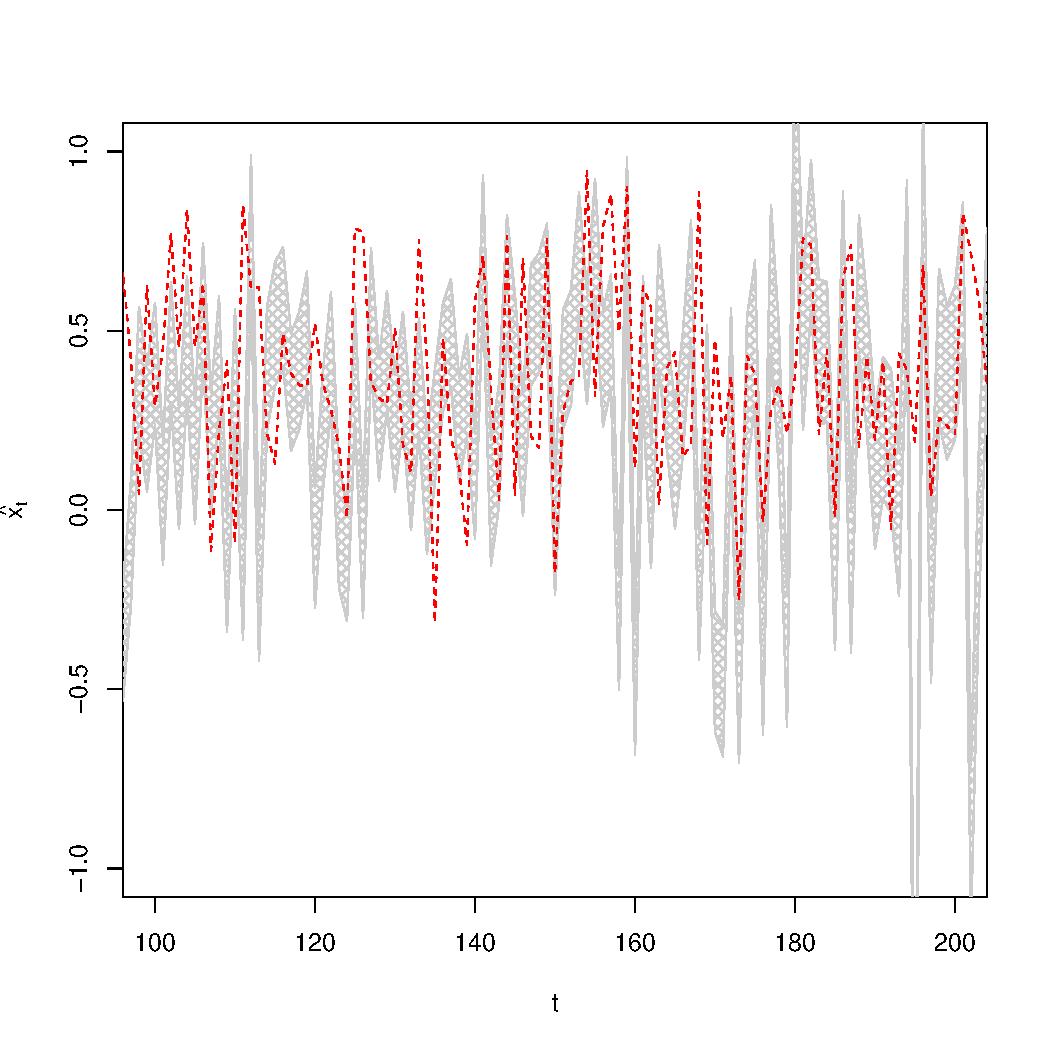
\includegraphics[height=7cm,width =10cm]{processo_1_01_02_05.pdf}
 \end{center}
\caption{Volatilidade estimada pelo modelo SV simulado entre $t \in [100 ;200]$. A região em cinza representa o intervalo de credibilidade ao nível de $95\%$ e em vermelho os valores verdadeiros.} 
\end{figure}

 \end{frame}
 
 
 \begin{frame}{SVM - parâmetros}

 
 \begin{figure}
\begin{center}
 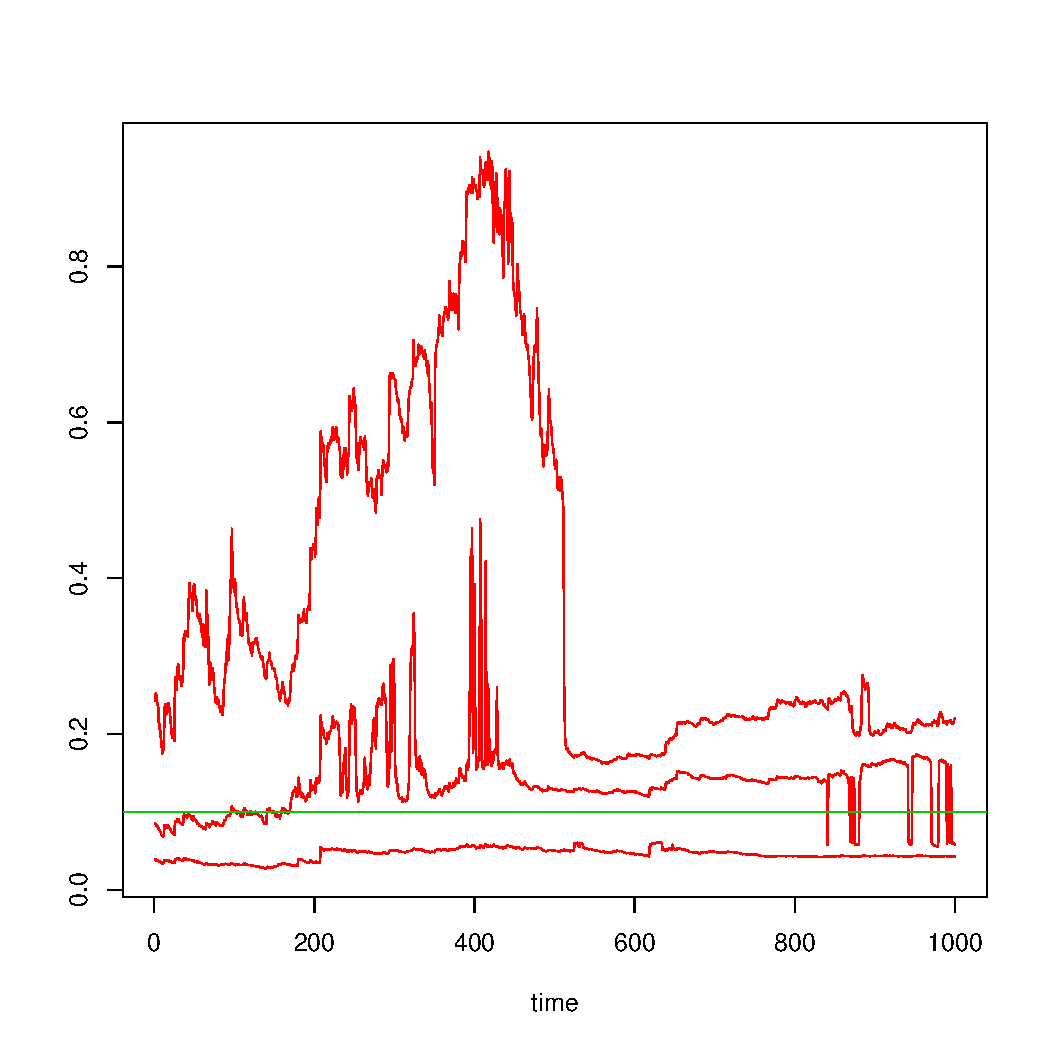
\includegraphics[height=7cm,width =10cm]{tau_1_01_02_05.pdf}
 \end{center}
\caption{ Estimativas dinâmicas para o parâmetro $\tau^2$.} 
\end{figure}

 \end{frame}
 



\begin{frame}{SVM - parâmetros}


 \begin{figure}
\begin{center}
 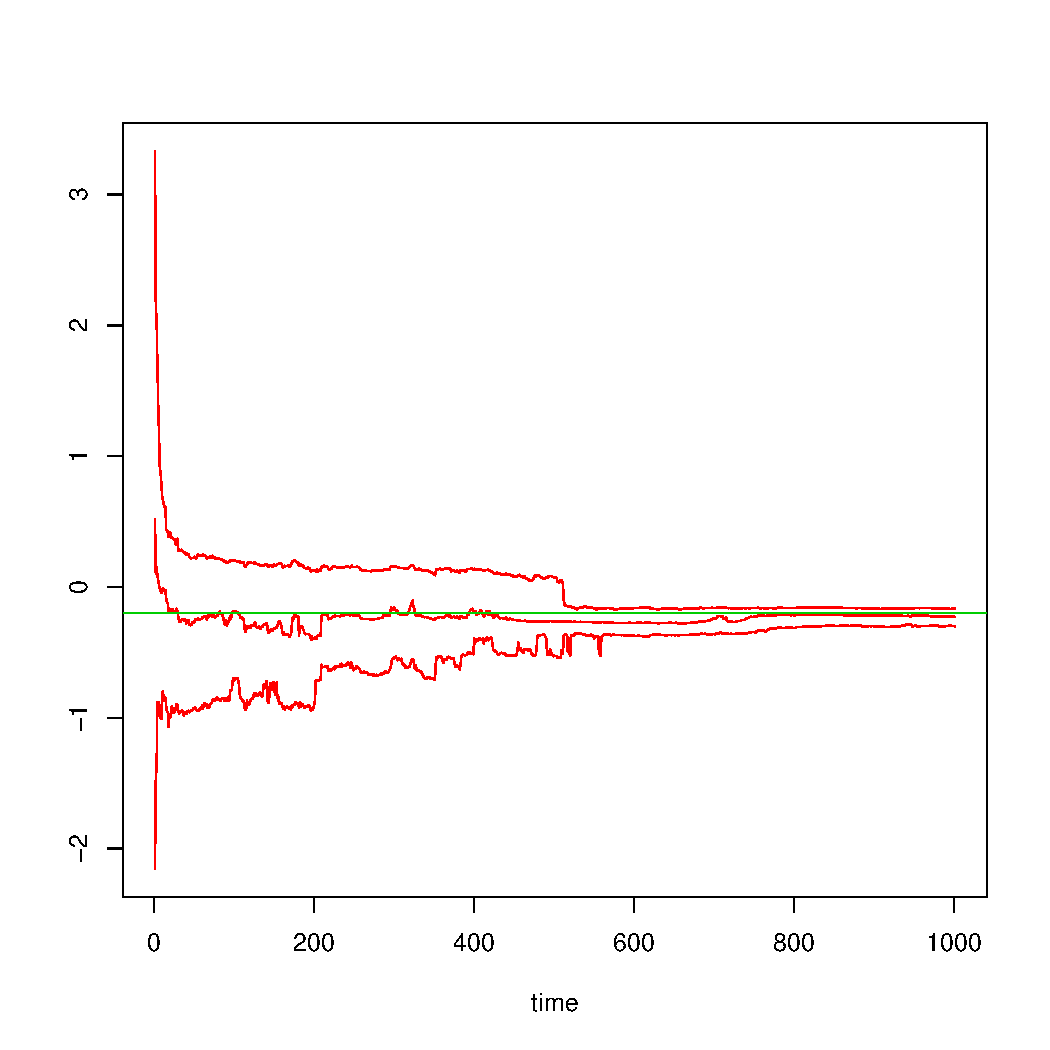
\includegraphics[height=7cm,width =10cm]{beta_1_01_02_05.pdf}
 \end{center}
\caption{Estimativas dinâmicas para o parâmetro $\beta$ } 
\end{figure}

 
 \end{frame}
 
 
 \begin{frame}{SVM - parâmetros}


 \begin{figure}
\begin{center}
 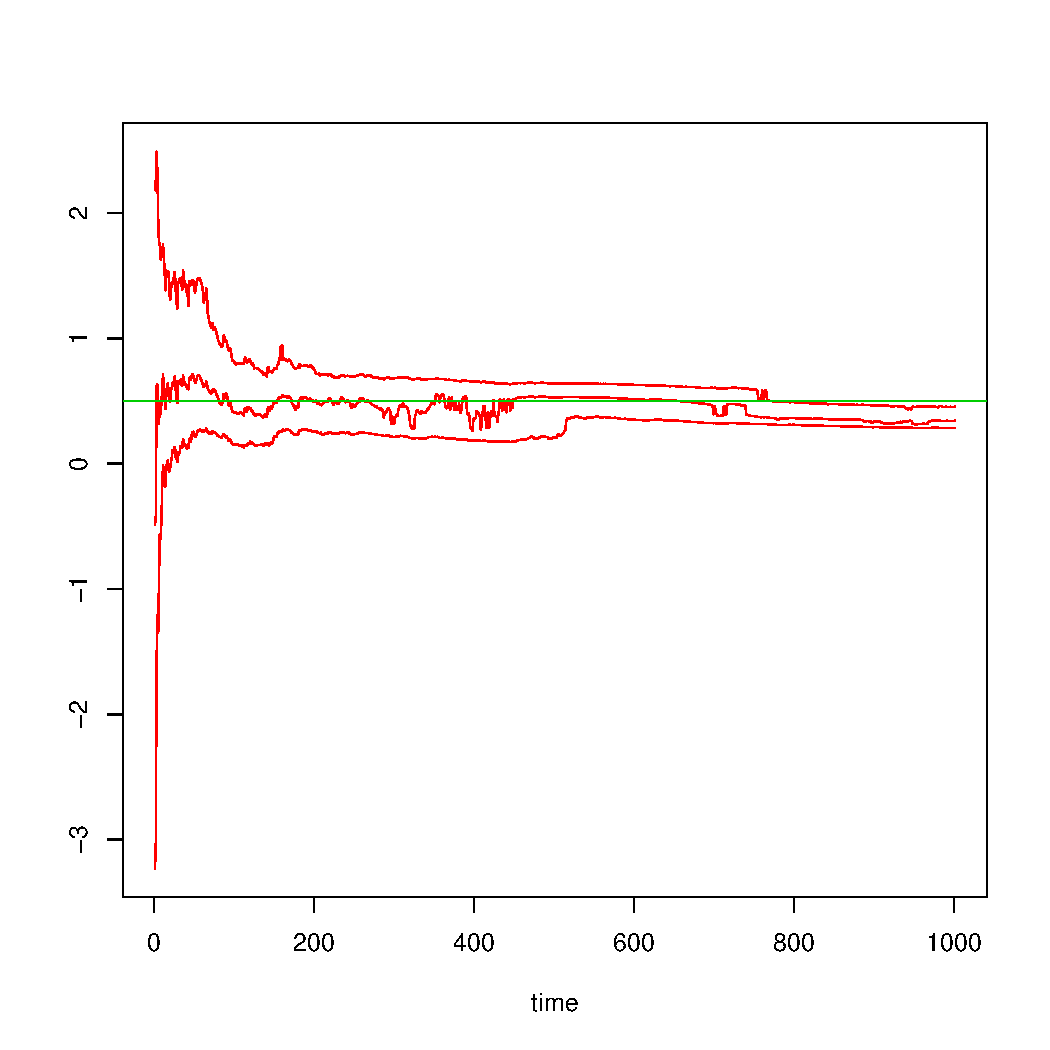
\includegraphics[height=7cm,width =10cm]{alpha_1_01_02_05.pdf}
 \end{center}
\caption{Estimativas dinâmicas para o parâmetro $\alpha$ } 
\end{figure}

 \end{frame}
 
 
 \begin{frame}{SVM - parâmetros}


% latex table generated in R 3.3.2 by xtable 1.8-2 package
% Tue Oct 31 22:24:28 2017
\begin{table}[ht]
\centering
\tiny
\begin{tabular}{c|cccc|cccc|cccc}
 \hline
  \hline
 & \multicolumn{4}{c|}{$\tau=\sqrt{0.1}=0.31$} &  \multicolumn{4}{c|}{$\beta=-0.2$} &  \multicolumn{4}{c}{$\alpha=0.5$} \\
 \hline
  & $\bar{\tau}$ & $\tilde{\tau}$ & $q_{5\%}$ & $q_{95\%}$ & $\bar{\beta}$ & $\tilde{\beta}$ & $q_{5\%}$ & $q_{95\%}$ & $\bar{\alpha}$ & $\tilde{\alpha}$ & $q_{5\%}$ & $q_{95\%}$\\ 
  \hline
Simulação & 0.34 & 0.24 & 0.21 & 0.45 & -0.23 & -0.23 & -0.29 & -0.17 & 0.34 & 0.34 & 0.29 & 0.44 \\ 
   \hline
    \hline
\end{tabular}
\caption[\scriptsize{Distribuição a posteriori de $\tau$, $\beta$ e $\alpha$}]{\scriptsize{Distribuição a posteriori dos hiperparâmetros nos modelos SV simulado com $M=5000$.}}
\label{tab:hiperest1000simula}
\end{table}

\end{frame}



 
\begin{frame}{}
    \begin{block}{ }
      \Huge  Aplicação
    \end{block}
\end{frame}

 
 \begin{frame}{Simulação}


Aplicação de R\$ $1000$ baseado nos dados $2008-2017$ dos ativos:
\vspace{.25cm}
\begin{itemize}
\item IFN:  índice setor financeiro
\item IMOB: índice do setor imobiliário
\item ICON: índice de consumo
\item IEE:  índice de energia
\item INDX: índice da indústria
\item IBOV: índice geral da bolsa de São Paulo
\item LTN: Letra do Tesouro Nacional
\end{itemize}
\vspace{.25cm}

Ajustar um modelo SV para cada série individualmente.
\end{frame}

\begin{frame}{IBOVESPA}



\begin{enumerate}
\item simulação de $10000$ carteiras aleatórias
\item $10000$ cenários
\item utilizando os parâmetros estimados para o modelo SV
\item $252$ períodos
\end{enumerate}


% latex table generated in R 3.3.2 by xtable 1.8-2 package
% Thu Nov 02 00:12:41 2017
\begin{table}[ht]
\centering
\tiny
\begin{tabular}{ccccccc|cccc}
   \hline
  \hline
 \multicolumn{7}{c|}{Alocação no ativo ($\%$)} &  \multicolumn{4}{c}{Valor final da carteira}\\
 \hline
ICON & IEE & IFN & IMOB & INDX & IBOV & LTN & $VaR_{99\%}$ & $VaR_{95\%}$ & $\bar{R}$  & $\sigma(W)$ \\ 
  \hline
11.21 & 2.67 & 11.81 & 1.27 & 35.79 & 9.16 & 28.09 & 624.84 & 711.95 & 7.50 & 241.79 \\ 
  34.27 & 2.89 & 11.98 & 16.57 & 2.97 & 1.78 & 29.54 & 597.63 & 733.85 & 8.34 & 242.06 \\ 
  34.35 & 0.66 & 7.85 & 2.53 & 0.79 & 25.12 & 28.71 & 633.07 & 728.82 & 8.08 & 249.42 \\ 
  17.78 & 0.86 & 10.60 & 15.77 & 23.91 & 5.93 & 25.14 & 607.13 & 711.50 & 6.27 & 251.81 \\ 
  20.13 & 2.77 & 5.07 & 13.93 & 6.28 & 20.94 & 30.89 & 611.37 & 701.44 & 7.00 & 254.07 \\ 
   \hline
      \hline
\end{tabular}
      \caption{\scriptsize{Informações das $5$ melhores carteiras no modelo SV independente. Análise de $10000$ carteiras, simuladas em $10000$ cenários de $252$ períodos.}}
\label{tab:carteirasim}
\end{table}

\end{frame}


 \begin{frame}{IBOVESPA}


\begin{itemize}
\item retorno médio esperado de $7.5\%$
\item \textit{VaR} ao nível $99\%$  de R\$ $624.84$
\item \textit{VaR} ao nível $95\%$ de R\$ $711.95$
\item pelo menos $25\%$ dos recursos alocados no ativo livre de risco.
\end{itemize}

\end{frame}




 \begin{frame}{Obrigado}

    
    \begin{center}
    
    \Huge{Perguntas?}
    
    \vspace{.75cm}
    
    \normalsize
    
    
    
    igor.ferreira.n@gmail.com
    
    \vspace{.25cm}
    
    lamfo.unb.br
    
    \vspace{.25cm}
    
    lamfo-unb.github.io
    
        
    \end{center}

\end{frame}




\begin{frame}[allowframebreaks]%in case more than 1 slide needed
    {\tiny
    \bibliography{bibli}
    }
\end{frame}

\end{document}



